\documentclass[oupdraft]{bio}
% \usepackage[colorlinks=true, urlcolor=citecolor, linkcolor=citecolor, citecolor=citecolor]{hyperref}
\usepackage{url}
\usepackage{hyperref} 
\usepackage{float}
% Add history information for the article if required
\history{}

\begin{document}

% Title of paper
\title{Enhancing comorbidity network inference with risk-enriched health trajectories embedding}

% List of authors, with corresponding author marked by asterisk
\author{Nicole Fontana$\ast$$^{1,2}$, Alessia Mapelli$\ast$$^{1,2}$, Emanuele Di Angelantonio$^{2}$, Francesca Ieva$^{1,2}$\\[4pt]
% Author addresses
\textit{$^1$MOX, Department of Mathematics, Politecnico di Milano, Milan, Italy}\\
\textit{$^2$Health Data Science Research Centre, Human Technopole, Milan, Italy}
\\[2pt]
% E-mail address for correspondence
{alessia.mapelli@polimi.it}\\
\textit{$^\ast$These authors contributed equally to this work.}}


% Running headers of paper:
\markboth%
% First field is the short list of authors
{N. Fontana and A. Mapelli}
% Second field is the short title of the paper
{Enhancing comorbidity network inference }

\maketitle

% Add a footnote for the corresponding author if one has been
% identified in the author list
\footnotetext{To whom correspondence should be addressed.}

\begin{abstract}
{Comorbidity networks provide crucial insights into disease relationships, yet traditional approaches relying on cross-sectional prevalence data face critical limitations: they overlook temporal disease progression, inadequately address confounding, and require arbitrary thresholding for network sparsification. We develop a comprehensive statistical framework that addresses these limitations through three methodological innovations. First, we adapt Word2Vec embeddings to longitudinal patient sequences, fine-tuning pretrained biomedical embeddings to learn representations that jointly encode temporal progression patterns and semantic disease relationships. Second, we introduce a confounding adjustment framework by jointly embedding diseases and risk factors, enabling explicit quantification of confounding by comparing risk-adjusted and unadjusted similarity networks. Third, we employ Gaussian Graphical Models with Lasso regularization to estimate conditional independence structure, providing sparsification without arbitrary thresholding. We apply this framework to UK Biobank data comprising 113,973 participants, focusing on 24 cardiometabolic diseases and 76 risk factors. The risk-adjusted network showed reduced connectivity among cardiometabolic diseases, indicating effective control for confounding effects. This finding was further confirmed by a validation analysis showing that pairs with larger changes in similarity systematically shared more risk factors. The analysis of the sparse network identified atrial fibrillation, acute kidney injury, and coronary disease as hub diseases with critical bridging functions. Community detection recovered three clinically meaningful modules aligned with established cardiometabolic taxonomy. Our framework demonstrates that integrating longitudinal data with explicit risk factor adjustment and advanced representation learning enhances the clinical validity of disease network analyses, providing a generalizable approach for more accurate characterization of multimorbidity patterns.}
{Comorbidity network; Longitudinal data; Word2Vec embeddings; Confounding adjustment; Gaussian Graphical Models; Cardiometabolic diseases}
\end{abstract}


\section{Introduction}\label{sec:introduction}
Multimorbidity, defined as the co-occurrence of two or more clinical conditions, has emerged as a critical challenge in modern healthcare systems. With aging populations and improved survival rates, its prevalence continues to rise, affecting approximately 25\% of adults and over 65\% of those aged 65 years or older~\citet{barnett2012epidemiology}. Cardiovascular and cardiometabolic diseases represent a particularly significant burden, accounting for nearly 18 million deaths annually worldwide and frequently presenting alongside metabolic, renal, and systemic disorders~\citet{roth2020global}. Understanding the complex patterns of disease co-occurrence and their underlying risk factors is essential for developing targeted prevention strategies, optimizing treatment protocols, and improving patient outcomes in complex clinical scenarios~(\citealp{PradosTorres2014, Yan2022}). %Moreover, characterizing these relationships can reveal shared underlying biological mechanisms and identify potential therapeutic targets that extend across multiple conditions. 

The study of comorbidity networks has gained substantial attention as a powerful framework for characterizing disease relationships~\citet{DelValle2019}. These networks represent diseases as nodes and their associations as edges, providing a systems-level view of multimorbidity patterns~\citet{Barabasi2011}. Traditional approaches to comorbidity network construction typically rely on cross-sectional prevalence or incidence data, where disease associations are computed as simultaneous presence rates within the study cohort at the specific time point~(\citealp{hidalgo2009dynamic, goh2007human}). Recent methodological advances have incorporated electronic health records and administrative databases to construct large-scale disease networks, leveraging statistical measures such as relative risk, odds ratios, phi-correlation, or Pearson correlation to quantify disease relationships~(\citealp{jensen2014temporal, siggaard2020disease, VargasFernandez2026Network, Burke2023}). While these methods have identified clinically meaningful disease clusters and progression pathways, they face three critical limitations.

First, most existing methods discard temporal information by using aggregate prevalence statistics or single time-point measurements~\citet{jeong2017network, dervic2025comorbidity}. Although some approaches incorporate longitudinal data for directed network construction, they typically rely on simple pairwise co-occurrence counts rather than learning representations that jointly capture temporal progression patterns and semantic disease relationships. This results in incomplete characterizations that fail to reflect the dynamic nature of multimorbidity development. Second, disease associations estimated solely from co-occurrence patterns are vulnerable to confounding by shared risk factors~(\citealp{vanderweele2013definition, pearl2009causality}). Two diseases may frequently co-occur not due to direct pathophysiological connections, but because they share common antecedents such as lifestyle factors or other comorbid conditions. Traditional network construction methods that ignore this confounding produce biased association estimates, artificially inflating similarities between diseases with shared risk profiles. Third, typical pair-wise estimation methods produce fully connected weighted networks that require arbitrary global thresholding for sparsification~\citet{masuda2025}. The resulting pruned networks depend critically on threshold selection, potentially removing clinically relevant connections while retaining spurious ones. Although statistical "backboning" methods have been proposed~(\citealp{serrano2009extracting, foti2011nonparametric}), these approaches assume heterogeneous weight distributions and often fail to extract meaningful structure from networks with relatively homogeneous similarity values.

%While graphical models can identify conditional dependencies, their application to disease network inference has not been combined with explicit risk factor adjustment in temporal sequence contexts.



To address these limitations, we develop a comprehensive statistical framework for disease network inference from longitudinal patient data that integrates three methodological innovations. First, we leverage complete longitudinal disease sequences as input, capturing the chronological progression of disease manifestations over the life course. We adapt Word2Vec embeddings, originally developed for natural language processing~\citet{mikolov2013efficient}, to longitudinal clinical sequences. We fine-tuned pretrained biomedical embeddings~\citet{zhang2019biowordvec} to learn dense vector representations that jointly encode temporal co-occurrence patterns and semantic disease relationships. Second, we introduce an approach to confounding adjustment by jointly embedding diseases and risk factors within a single representation space. This is motivated by the distributional principle underlying Word2Vec-style models, where incorporating additional relevant context reshapes the local co-occurrence neighborhoods used for training, leading to richer and more informative semantic representations. We explicitly evaluated this reshaping by comparing risk-adjusted and unadjusted similarity networks to quantify confounding effects. We validate confounding removal by demonstrating that disease pairs with larger similarity changes systematically share more risk factors, confirming that observed decreases reflect genuine confounding adjustment rather than noise. Third, we employ Gaussian Graphical Models (GGM) with Lasso regularization~\citet{meinshausen2006high} to achieve network sparsification by estimating conditional independence structure, identifying direct disease associations while removing indirect relationships mediated through other diseases or risk factors. This conditional independence framework provides a statistically rigorous alternative to arbitrary thresholding, naturally producing sparse networks suitable for topological analysis and identification of hub diseases, improving clinical interpretability.

We apply this framework to construct a cardiometabolic comorbidities disease network using longitudinal data from UK Biobank, incorporating 24 primary cardiometabolic diseases and 76 risk factors. Our results demonstrate substantial confounding, with 91.3\% of disease pairs showing decreased association after risk adjustment. The sparse GGM-derived network preserves established pathophysiological relationships while revealing hub diseases with both high epidemiological burden and critical bridging functions between distinct biological domains. 

The remainder of this paper is structured as follows. Section~\ref{sec:data} describes the UK Biobank cohort, phenotype definitions, and data preprocessing. Section~\ref{sec:method} presents our methodological framework, including sequence construction, word embedding strategy, similarity-based network construction, confounding evaluation, and GGM-based sparsification. Section~\ref{sec:results} reports results for cardiometabolic disease networks, including confounding quantification and topological analysis. Section~\ref{sec:discussion} discusses methodological implications, limitations, and future directions.

\section{Data and phenotype definition}\label{sec:data}
%\subsection{The UK Biobank cohort}
The UK Biobank is a large-scale prospective cohort study comprising approximately 500,000 participants aged 40-69 years at recruitment between 2006 and 2010 across the United Kingdom~\citet{Sudlow2015UKBiobank}. This population-based resource represents one of the most comprehensive biomedical databases worldwide, systematically integrating demographic information, lifestyle questionnaires, physical measurements, biological samples, multi-omics data, and longitudinal electronic health record (EHR) linkage. The core of our analytical framework resides in the definition of a high-dimensional phenotyping space, designed to capture the longitudinal evolution of cardiometabolic conditions. We defined 24 primary cardiometabolic diseases as the core focus of the comorbidity network, alongside 76 risk factors selected based on established epidemiological literature. Phenotype definitions were developed through expert clinical consultation to ensure consistency with diagnostic criteria and epidemiological standards. We adopted a multi-source ascertainment strategy that integrates three distinct clinical domains: ICD-10 diagnosis codes and OPCS-4 procedure codes indicating surgical or interventional treatment (1) from hospital inpatient records; (2) from primary care data; and (3) laboratory measurements from primary care data. This multi-source definition strategy enhances phenotype sensitivity by capturing patients' history through diverse clinical touchpoints. The 24 primary diseases encompass major cardiovascular conditions (acute myocardial infarction, coronary disease, heart failure, atrial fibrillation, ventricular arrhythmias, cardiac arrest, cardiomyopathies), valvular heart diseases (aortic, mitral, and tricuspid valve disorders), vascular diseases (cerebrovascular disease, hemorrhagic stroke, aneurysm and dissection, peripheral vascular diseases, acute pulmonary embolism), advanced cardiovascular interventions (pacemaker implantation for conduction delay, heart transplantation for end-stage heart failure), metabolic conditions (diabetes mellitus, dyslipidemias), hypertension, and progressive stages of renal dysfunction (acute kidney injury, chronic kidney disease stages 3-5, end-stage renal disease). In addition to the primary diseases, 76 risk factors were considered to adjust for confounding, including demographic and socioeconomic factors, family history of cardiovascular disease, lifestyle and anthropometric factors, clinical biomarkers, and comorbidities. Complete definitions and life-course incidences for each disease are provided in Supplementary Table~\ref{ST:table1} for the primary diseases and Supplementary Table~\ref{ST:table2} for risk factors. Longitudinal incidence distribution plots for each primary disease are shown in Supplementary Figure~\ref{supp_mat:SF0}. All phenotypes were mapped to the Medical Subject Headings (MeSH) vocabulary to enable integration with BioWordVec pretrained embeddings. After MeSH mapping, the final vocabulary comprised 24 unique main diseases and 76 unique risk factors (98 unique events). Information about the MeSH mapping is provided in Supplementary Tables~\ref{ST:table1} and~\ref{ST:table2}. We recorded 544,716 primary disease events and 3,285,210 risk factor events, with Figure~\ref{fig:main_dist_time_events_SF3} showing the temporal distribution of the disease events. Starting from 502,297 UK Biobank participants, we excluded individuals with fewer than three recorded main disease events during the life course. The final cohort comprised 113,973 participants. For each participant, we constructed longitudinal event sequences capturing temporal progression throughout their clinical history; details are provided in Section~\ref{subsection:seq_con}. %Phenotype terms were mapped to Medical Subject Headings (MeSH) vocabulary to enable integration with BioWordVec pretrained embeddings. %During MeSH mapping, Endstage Heart Failure and Heart Failure were consolidated into a single term. 

\begin{figure}
    \centering
    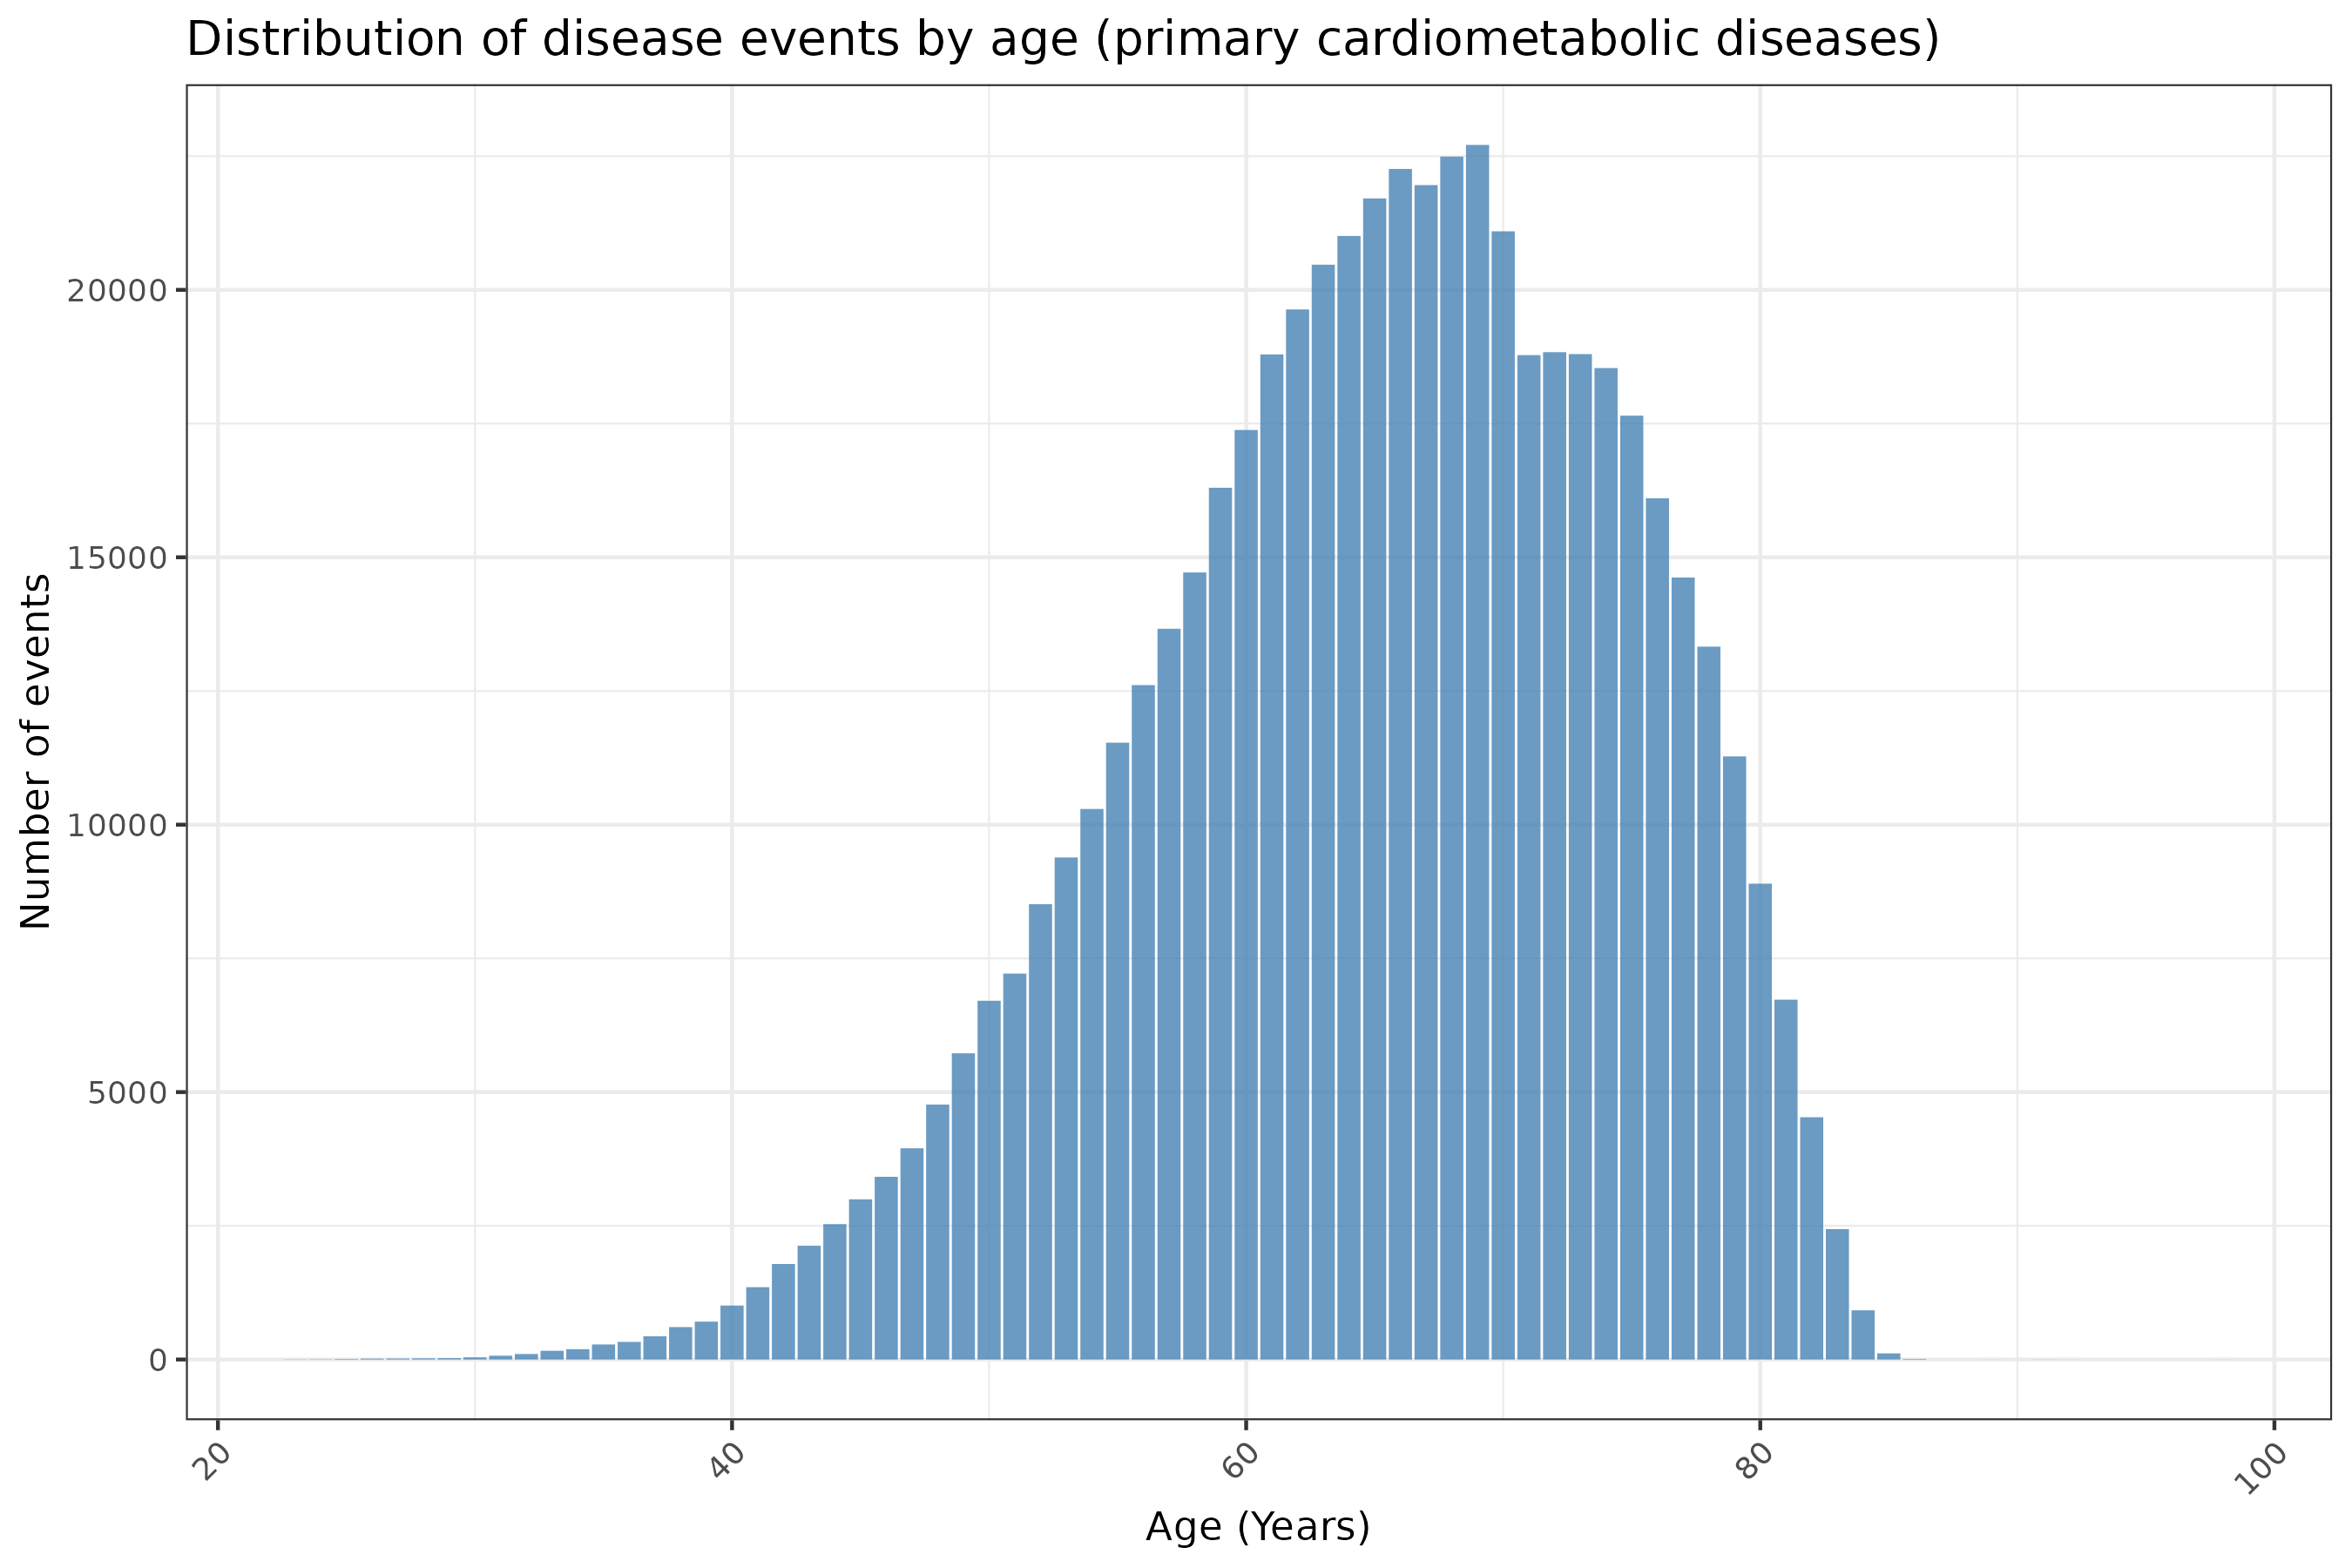
\includegraphics[width=\linewidth]{Figures/total_events_by_age.png}
        \caption{Distribution of event times for 24 primary cardiometabolic diseases.}
        \label{fig:main_dist_time_events_SF3}
\end{figure}



\section{Method}\label{sec:method}
We address the problem of estimating disease comorbidity networks from longitudinal patient event sequences while adjusting for confounding by shared risk factors. To reach this goal, we model disease relationships using an undirected weighted graph $G=(V,E)$, where the node set $V$ represents diseases and the edge set $E$ encodes pairwise associations. Edge weights are stored in the weighted adjacency matrix $A$, whose entries $A_{ij}$ quantify the strength of the relationship between diseases $i$ and $j$ based on their co-occurrence and temporal ordering within patient trajectories. Our methodological pipeline, shown in Figure~\ref{fig:pipeline}, consists of six main stages, each addressing a key challenge in translating longitudinal patient data into interpretable disease networks. First in Section~\ref{subsection:seq_con}, we construct temporally ordered event sequences from patient histories to preserve chronological information that is lost in traditional prevalence-based approaches. Second in Section~\ref{subsection:word_embedding}, we learn dense vector representations of diseases and risk factors by adapting pretrained Word2Vec embeddings to longitudinal clinical data, enabling representations that capture both temporal context and biomedical semantics. Third, in Section~\ref{subsection:network_con} we construct dense disease similarity networks using cosine similarity between learned embeddings, yielding weighted networks that encode global semantic and temporal relationships among diseases. Fourth in Section~\ref{subsection:risk_factor}, we introduce a principled framework to evaluate and correct confounding induced by shared risk factors, enabling the derivation of adjusted disease similarity networks that better reflect direct pathophysiological relationships. Finally, in Sections~\ref{subsec:sparsification} and~\ref{subsec:topology}, we apply Gaussian Graphical Models with Lasso regularization to obtain sparse networks that capture conditional dependencies, facilitating interpretability, visualization, and topological analysis.

\begin{figure}[t]
    \centering
    \hspace*{-1.8cm}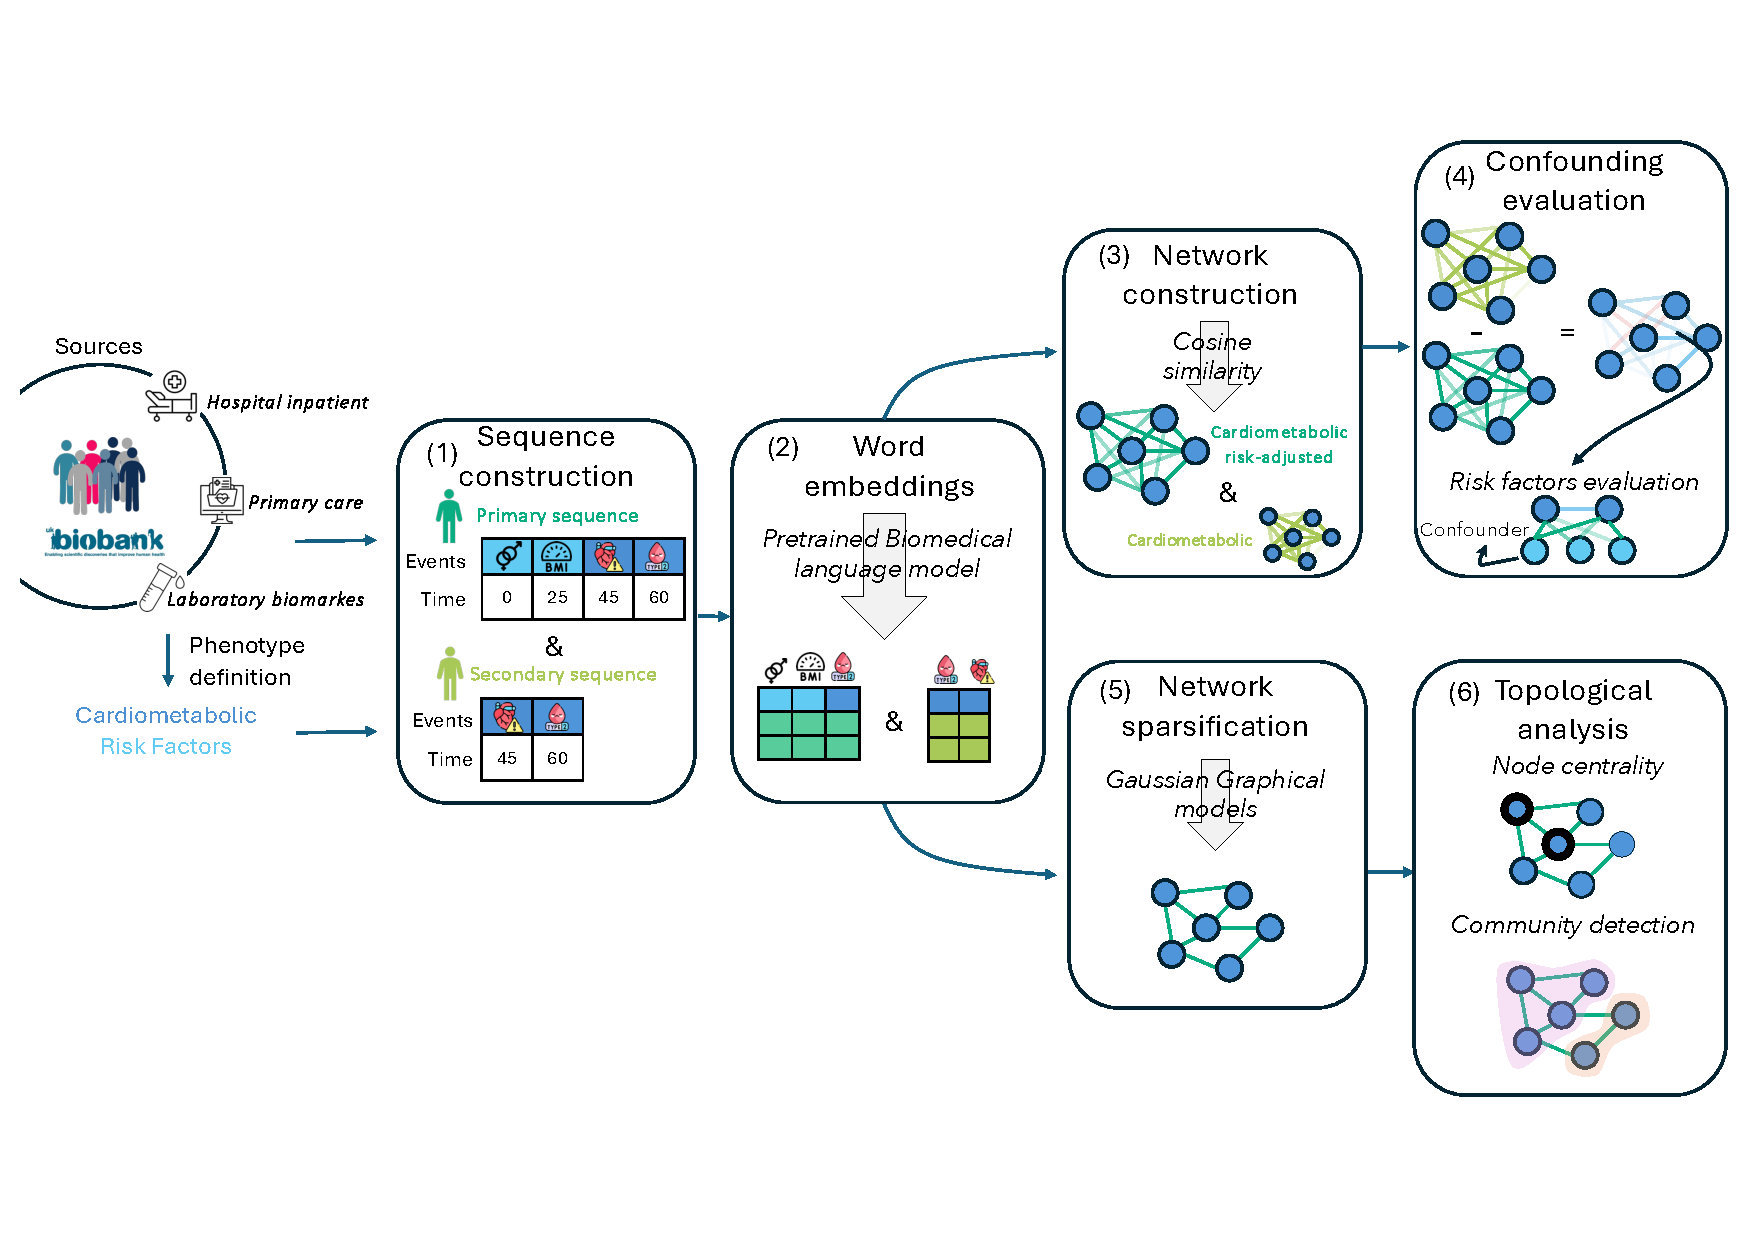
\includegraphics[width=1.3\linewidth]{Figures/pipeline.pdf}
    \caption{Schematic representation of the methodological framework for risk-adjusted cardiometabolic comorbidity network inference. The workflow proceeds through four primary stages: (1) Phenotype definition and sequence construction: integration of multimodal data sources, including hospital records, primary care data, and clinical biomarkers, to generate a primary sequence including both cardiometabolic diseases and risk factors and a secondary sequence restricted to cardiometabolic diseases. (2) Word embeddings: mapping of clinical events into a dense vector space by fine-tuning pretrained biomedical language models on cohort-specific patient sequences. (3-4) Network construction and confounding evaluation: estimation of pairwise cosine similarities to quantify disease associations and implementation of a systematic comparison between unadjusted and risk-adjusted networks to identify and remove confounding effects. (5-6) Network sparsification and topological analysis: sparse network construction via Gaussian Graphical Models to identify direct conditional dependencies, followed by the characterization of central disease hubs and the detection of disease modules through modularity optimization.}
    \label{fig:pipeline}
\end{figure}

\subsection{Sequence construction}\label{subsection:seq_con}
For each patient $p \in \{1, \ldots, P\}$, we construct a temporal event sequence:
\begin{equation}
S_p = \{(t_1, v_1), (t_2, v_2), \ldots, (t_{n_p}, v_{n_p})\},
\end{equation}
where $n_p$ denotes the number of recorded events, $v_j \in \mathcal{V}$ represents the event identifier (disease or risk factor), and $t_j \in \mathbb{R}_+$ denotes time from birth in days. Sequences are ordered chronologically such that $t_1 < t_2 < \cdots < t_{n_p}$. This temporal ordering enables the embedding model to capture both co-occurrence patterns and disease progression dynamics. We construct a primary sequence $S_p^{(\mathcal{D}+\mathcal{R})}$ containing events from the full vocabulary $\mathcal{V} = \mathcal{D} \cup \mathcal{R}$, where $\mathcal{D}$ denotes the set of cardiometabolic diseases and $\mathcal{R}$ the set of risk factors, yielding a vocabulary size $|\mathcal{V}^{(\mathcal{D}+\mathcal{R})}| = 122$. To evaluate the effect of risk factor adjustment, we also construct a secondary sequence $S_p^{(\mathcal{D})}$, restricted to cardiometabolic diseases, with vocabulary size $|\mathcal{V}^{(\mathcal{D})}| = D = 24$. In the following, we denote events $v_j \in \mathcal{D}$ by $d_j$ and events $v_j \in \mathcal{R}$ by $r_j$.

\subsection{Word embeddings}\label{subsection:word_embedding}
In natural language processing, representation learning maps words into a continuous, low-dimensional embedding vector space where geometric proximity reflects semantic similarity derived from contextual co-occurrence. We adapt the Word2Vec skip-gram architecture to longitudinal clinical data by conceptualizing medical events as ``words'' and entire patient trajectories as ``sentences''. The choice of this framework is motivated by the ability of Word2Vec to generate embeddings, in which entities appearing in similar clinical contexts, such as conditions with shared pathophysiological precursors, are mapped closely in the embedding space. This approach enables the efficient extraction of information from complex longitudinal sequences without increasing model complexity, effectively balancing representational power with computational efficiency. We leverage the pretrained BioWordVec model~\citet{zhang2019biowordvec}, which combines embeddings trained on 27 million PubMed abstracts with Medical Subject Headings (MeSH) structure, providing domain-specific biomedical knowledge. Each phenotype is tokenized into constituent words (e.g., ``Chronic Kidney Disease'' $\rightarrow$ [``Chronic'', ``Kidney'', ``Disease'']). We fine-tune BioWordVec on patient sequences using the original skip-gram configuration: embedding dimension $d=200$, context window size $c=5$, and standard learning rate schedule. To balance cohort-specific adaptation with preservation of biomedical semantics, we monitor the cosine similarity between pretrained and fine-tuned embeddings:
\begin{equation}
\text{sim}_{\text{preserved}}^{(t)} = \frac{1}{|\mathcal{V}|} \sum_{v \in \mathcal{V}} \frac{\mathbf{e}_v^{(t)} \cdot \mathbf{e}_v^{(0)}}{\|\mathbf{e}_v^{(t)}\| \|\mathbf{e}_v^{(0)}\|},
\end{equation}
where $\mathbf{e}_v^{(t)}$ denotes the embedding at epoch $t$ and $\mathbf{e}_v^{(0)}$ the pretrained embedding. Fine-tuning is stopped when $\text{sim}_{\text{preserved}}^{(t)} < 0.70$, ensuring at least $70\%$ semantic retention. In our application, this criterion was satisfied after 4 epochs. For phenotypes composed of multiple words (e.g., ``Chronic Kidney Disease"), let $W$ be the set of constituent tokens (e.g., $W \in \{\text{``Chronic"; ``Kidney"; ``Diseases"}\}$). The phenotype embedding is computed as the average:
\begin{equation}
\mathbf{e}_{\text{phenotype}} = \frac{1}{|\text{$W$}|} \sum_{w \in \text{$W$}} \mathbf{e}_w.
\end{equation}

\subsection{Network construction using cosine similarity}\label{subsection:network_con}
Following established practices in the literature~\citet{gundougan2020research}, to determine the relationship between phenotype embeddings and construct the weighted adjacency matrix $A$, we used pairwise cosine similarity. Given phenotype embeddings $\{\mathbf{e}_1, \ldots, \mathbf{e}_D\}$, the adjacency matrix $A \in [0,1]^{D \times D}$ is defined as:
\begin{equation}\label{eq:cosine_similarity}
A_{ij} = \text{sim}(\mathbf{e}_i, \mathbf{e}_j) = \frac{\mathbf{e}_i \cdot \mathbf{e}_j}{\|\mathbf{e}_i\| \|\mathbf{e}_j\|}.
\end{equation}
This produces a fully connected, weighted network where edge weights reflect overall semantic and contextual similarity between diseases. Cosine similarity ranges from $-1$ (opposite identical) to $+1$ (identical), with values near 0 indicating orthogonality in the embedding space (no shared meaning). We construct two disease similarity networks: $A^{(\mathcal{D}+\mathcal{R})}$, derived from embeddings learned from the primary sequences containing both cardiometabolic diseases and risk factors, and $A^{(\mathcal{D})}$, derived from embeddings trained on the secondary disease-only sequences.

\subsection{Confounding evaluation}\label{subsection:risk_factor}
\subsubsection{Conceptual framework}
We define confounding in the embedding space as follows: if diseases $d_i, d_j \in \mathcal{D}$ are associated in patient trajectories due to a share common risk factor $r_k \in \mathcal{R}$, then similarity computed from disease-only sequences, $A_{ij}^{(\mathcal{D})}$, is expected to be inflated related to the ``true" pathophysiological relationship. Jointly embedding diseases and risk factors redistributes part of this shared signal to the risk factor dimensions, yielding adjusted disease embeddings and corrected similarity estimates $A_{ij}^{(\mathcal{D}+\mathcal{R})}$.

\subsubsection{Statistical evaluation of changes}
We quantify similarity changes as:
\begin{equation}\label{eq:similarity_difference}
\Delta_{ij} = A_{ij}^{(\mathcal{D}+\mathcal{R})} - A_{ij}^{(\mathcal{D})}.
\end{equation}
Negative values ($\Delta_{ij} < 0$) indicate confounding removal (similarity decreased after adjustment), while positive values ($\Delta_{ij} > 0$) suggest unmasking of true relationships previously obscured by noise. We assess the global impact of risk adjustment using the Mean Absolute Difference (MAD) to quantify the average magnitude of change across all disease pairs and the Mean Directional Change (MDC) to assess systematic bias in adjustment direction: 
\begin{equation}
\text{MAD} = \frac{1}{D(D-1)/2} \sum_{i < j} |\Delta_{ij}|,\text{ } \text{ } \text{ } \text{MDC} = \frac{1}{D(D-1)/2} \sum_{i < j} \Delta_{ij},
\end{equation}
where negative MDC indicates systematic similarity decreases. We employed a Wilcoxon signed-rank test to test the null hypothesis $H_0: \text{median}(\Delta_{ij}) = 0$ against the alternative $H_1: \text{median}(\Delta_{ij}) \neq 0$, providing formal statistical evidence of systematic change. To evaluate preservation of network structure, we compute the Spearman rank correlation:
\begin{equation}
\rho_S = \text{corr}_{\text{Spearman}}(\{A_{ij}^{\mathcal{D}}\}_{i<j}, \{A_{ij}^{\mathcal{D+R}}\}_{i<j}),
\end{equation}
where a high correlation ($\rho_S \approx 1$) indicates structural preservation despite local adjustments.

\subsubsection{Confounding detection and validation}\label{subsub:conf_det}
To validate that observed similarity changes reflect genuine confounding removal rather than random noise, we implement a three-step analysis linking similarity changes to shared risk factors:

\textbf{Step 1: Identify highly affected pairs.} Disease pairs are ranked by $|\Delta_{ij}|$, and those in the 95-$th$ percentile of the distribution are selected.

\textbf{Step 2: Identify disease-risk factor associations.} For each disease $d_i \in \mathcal{D}$, associated risk factors $\mathcal{R}_i \subset \mathcal{R}$ are identified based on their embedding similarity. A risk factor $r \in \mathcal{R}$ is considered associated with disease $d_i \in \mathcal{D}$ if:
\begin{equation}\label{eq:rf_threshold}
\text{sim}(\mathbf{e}_{d_i}, \mathbf{e}_{r}) > \tau,
\end{equation}
where $\tau$ is the median pairwise similarity among all risk factors: 
\begin{equation} \tau = \text{median} \left( { \text{sim}(\mathbf{e}_{r_k}, \mathbf{e}_{r_l}) : 1 \le k < l \le R } \right). 
\end{equation}
This threshold ensures that only associations that are strong, relative to the global correlation structure induced by the risk factors' embedding, are further investigated.

\textbf{Step 3: Quantify shared risk factors.}
For disease pair $(d_i, d_j)$, the proportion of shared risk factors is computed as:
\begin{equation}\label{eq:shared_rf}
\text{SharedRF}_{ij} = \frac{|\mathcal{R}_i \cap \mathcal{R}_j|}{min(|\mathcal{R}_i|, | \mathcal{R}_j|)}.
\end{equation}
Under our confounding framework, high $|\Delta_{ij}|$ values are expected to correspond to large $\text{SharedRF}_{ij}$. To formally test this hypothesis, we use a Mann-Whitney U test to evaluate whether the distribution of $\text{SharedRF}_{ij}$ is stochastically greater in highly affected pairs (defined in Step 1) against that of all remaining pairs. A significant result would provide statistical evidence that confounding magnitude correlates with shared risk factor burden, validating our adjustment procedure.

Finally, to assess the robustness of the choice of the confounding detection threshold $\tau$, we repeat the analysis in a range of $\tau \in \{0.5, 0.6, 0.7, 0.8, 0.9\}$ and report for each threshold the proportion of shared risk factors in the highly affected pairs and the Mann-Whitney U test.

\subsection{Network sparsification using Gaussian Graphical Models}\label{subsec:sparsification}
Similarity-based networks are inherently fully connected, while this weighted adjacency matrix contains the complete set of pairwise relationships, the underlying structural properties are often obscured by the high edge density, complicating visualization, interpretation, and topological inference. Conventionally, sparsification is achieved by applying a global hard threshold, where edges are retained only if their weights exceed an arbitrary value. To move beyond such heuristic approaches, statistical "backboning" methods have been proposed to identify edges that are significantly stronger than a null model~\citet{foti2011nonparametric}. However, these methods typically assume a high degree of heterogeneity in the weight distribution and they fail to extract a meaningful latent geometry in fully connected networks where similarity values are relatively homogeneous or narrowly distributed. Consequently, to obtain a sparse and interpretable representation, we adopt a Gaussian Graphical Model (GGM) framework. Unlike cosine similarity, which captures overall contextual relatedness, a GGM estimates partial correlations that quantify the association between two diseases after conditioning on the influence of all other variables in the system. This approach provides a principled mechanism for direct sparsification through Lasso regularization, effectively pruning edges that do not represent direct conditional dependencies. A more detailed discussion on the limitations of traditional backboning methods in this context is provided in Supplementary Method~\ref{supp_met_1}.

Treating each embedding dimension as an independent observation~\citet{zhelezniak2019correlation}, the embedding vectors $\{\mathbf{e}_v\}_{v \in \mathcal{V}}$ are assumed to follow a multivariate Gaussian distribution $
\mathbf{e} \sim \mathcal{N}(\boldsymbol{\mu}, \boldsymbol{\Sigma})
$
where $\boldsymbol{\Sigma} \in \mathbb{R}^{(D+R) \times (D+R)}$ is the covariance matrix. Under this hypothesis, conditional independence is encoded in the precision matrix $\boldsymbol{\Omega} = \boldsymbol{\Sigma}^{-1}$ with $\omega_{ij} = 0$ if and only if embeddings $i$ and $j$ are conditionally independent given all other events. The multivariate normality assumption was evaluated using Shapiro-Wilk tests on each embedding dimension, with a significance threshold $\alpha = 0.05$. We employ a neighborhood selection approach~\citet{meinshausen2006high} to estimate $\boldsymbol{\Omega}$ through $D+R$ independent Lasso regression models. For each phenotype $i \in \mathcal{D \cup R}$, we solve:
\begin{equation}\label{eq:neighborhood_selection}
\hat{\boldsymbol{\beta}}^{(i)} = \mathop{\arg \min}_{\boldsymbol{\beta} \in \mathbb{R}^{R+D-1}} \|\mathbf{e}_i - \mathbf{E}_{-i}\boldsymbol{\beta}\|_2^2 + \lambda \|\boldsymbol{\beta}\|_1,
\end{equation}
where $\mathbf{E}_{-i}$ is the matrix of embeddings excluding phenotype $i$, and $\lambda > 0$ controls sparsity through the $\ell_1$ penalty. The estimated neighborhood of phenotype $i$ is:
\begin{equation}
\hat{E}_i = \{j : \hat{\beta}_j^{(i)} \neq 0 \text{ or } \hat{\beta}_i^{(j)} \neq 0\},
\end{equation}
using the OR rule to ensure symmetry. The binary adjacency matrix is then obtain as:
\begin{equation}\label{eq:ggm_adjacency}
A_{ij}^{\mathcal{(D+R)}} = \mathbb{I}(j \in \hat{E}_i).
\end{equation}
The regularization parameter $\lambda$ is selected via 10-fold cross-validation, minimizing mean squared prediction error.


\subsection{Network topology analysis}\label{subsec:topology}
To characterize the systemic importance of individual diseases and uncover the modular architecture of the cardiometabolic landscape, we performed a topological analysis on the sparse GGM-derived network. We quantified disease importance using two complementary centrality measures, each capturing a distinct aspect of clinical relevance within the comorbidity network. Degree centrality ($C_D$) assesses the local connectivity of a node by quantifying the number of its direct disease associations:
\begin{equation}
C_D(i) = \sum_{j=1}^D A_{ij}.
\end{equation}
Betweenness centrality ($C_B$) serves as a global measure of a node's influence by identifying diseases that bridge distinct pathophysiological domains:
\begin{equation}
C_B(i) = \sum_{s \neq i \neq t} \frac{\sigma_{st}(i)}{\sigma_{st}},
\end{equation}
where $\sigma_{st}$ denotes the total number of shortest paths between diseases $s$ and $t$, and $\sigma_{st}(i)$ is the subset of those paths passing through disease $i$. 

Finally, we identified cohesive disease modules by applying the fast greedy modularity optimization algorithm~\citet{clauset2004finding}. This approach partitions the network into communities by maximizing the modularity $Q$:
\begin{equation}
Q = \frac{1}{2m} \sum_{ij} \left(A_{ij} - \frac{C_D(i) C_D(j)}{2m}\right) \delta(c_i, c_j),
\end{equation}
where $m = \frac{1}{2}\sum_{ij} A_{ij}$ represents the total edge count, $c_i$ denotes the community assignment of node $i$, and $\delta(c_i, c_j) = 1$ if $c_i = c_j$ and 0 otherwise. The algorithm iteratively merges communities to maximize $Q$, producing a hierarchical dendrogram. We select the partition with maximum modularity as the final community structure.

\section{Results}\label{sec:results}
We applied our methodological framework to construct cardiometabolic comorbidity networks from UK Biobank longitudinal data. Our analysis proceeds in three stages: in Section~\ref{subsubsection:res_cosine}, we construct and validate the cardiometabolic risk-adjusted disease similarity network; in Section~\ref{subsubsection:results_conf}, we quantify confounding effects by comparing the primary risk-adjusted with the disease-only network; in Section~\ref{subsubsection:topology}, we apply GGM-based networks for sparsification and perform topological analysis. All analyses use as input embeddings extracted from the fine-tuned BioWordVec model detailed in Section~\ref{subsection:word_embedding}.

\subsection{Cardiometabolic risk-adjusted disease similarity network}\label{subsubsection:res_cosine}
The risk-adjusted cardiometabolic disease network, constructed by computing cosine similarities between disease embeddings fine-tuned on primary sequences, is shown as an adjacency matrix in Figure~\ref{fig:disease_similarity_heatmap_main_par}, with the corresponding graph visualization provided in Supplementary Figure~\ref{supp_mat:SF2}. This network constitutes our primary result, as it explicitly accounts for confounding due to shared risk-factor profiles through the joint embedding framework.

\begin{figure}[h]
    \centering
    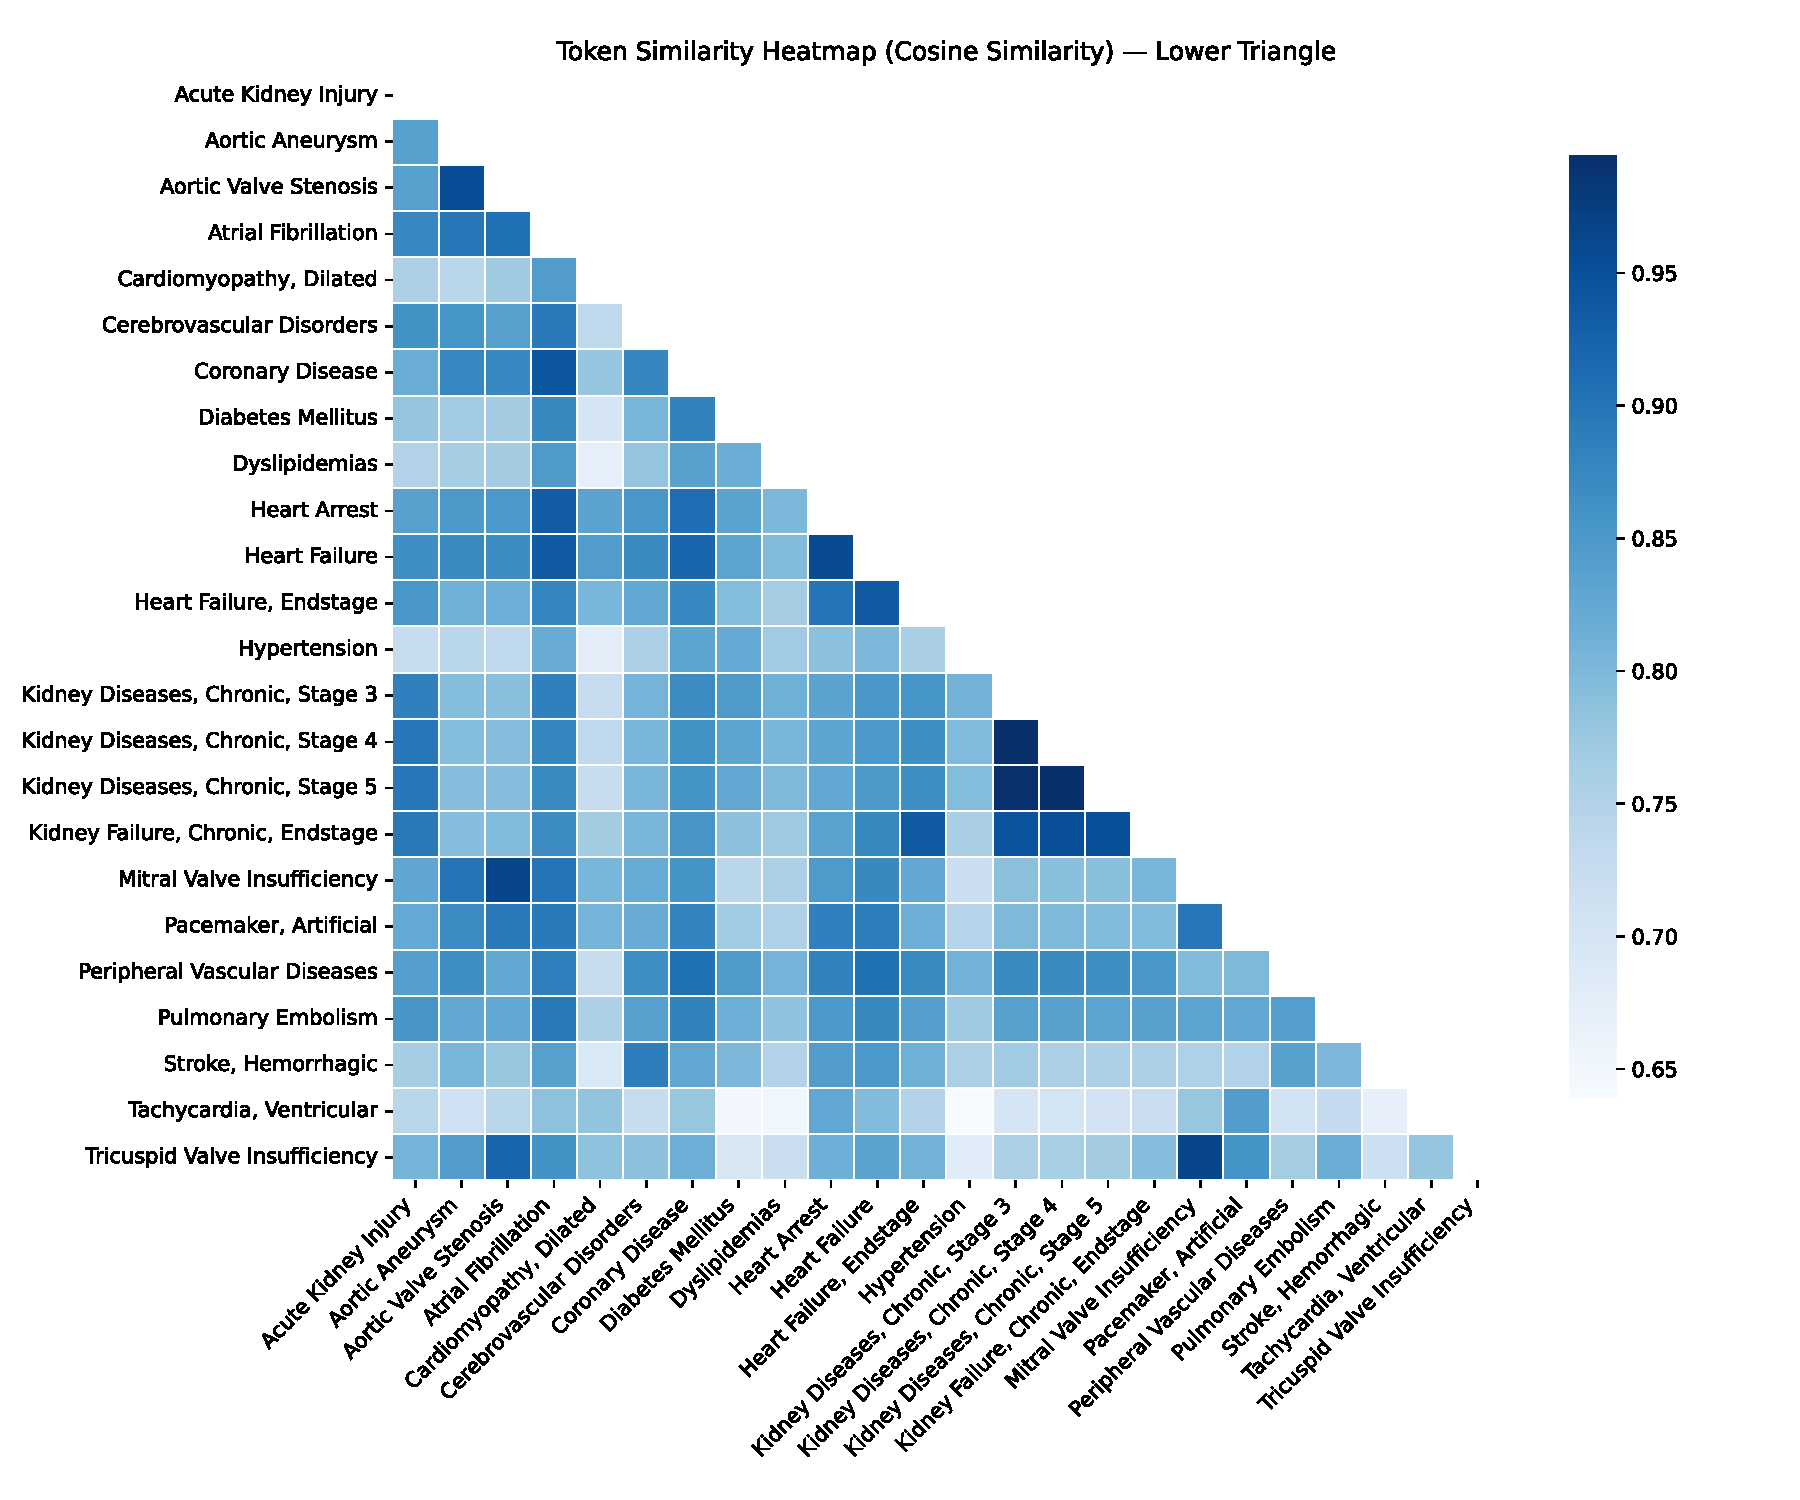
\includegraphics[width=0.9\textwidth]{Figures/disease_similarity_heatmap_main_par.pdf}
    \caption{Cosine similarity matrix for 24 cardiometabolic diseases computed from embeddings including both cardiometabolic diseases and risk factors. Darker colors indicate stronger similarities. The graph visualization is provided in Figure~\ref{supp_mat:SF2}.}
    \label{fig:disease_similarity_heatmap_main_par}
\end{figure}
The resulting adjacency matrix reveals clinically meaningful disease clusters consistent with established pathophysiological mechanisms. The chronic kidney disease (CKD) pathway emerges as a prominent domain, with strong connections between progressive renal dysfunction stages and end-stage renal disease. Acute kidney injury shows notable associations with this progression pathway, reflecting the well-documented transition from acute renal impairment to chronic dysfunction~\citet{chawla2014acute}. 
The strong similarity between heart failure and CKD stages is consistent with the cardiorenal syndrome framework, in which hemodynamic alterations, activation of the renin–angiotensin–aldosterone system, and fluid overload contribute to a bidirectional progression of disease~\citet{ronco2008cardiorenal}.
A cohesive valvular disease module emerges within the network, capturing the intrinsic dependencies among mitral, tricuspid, and aortic valve disorders. In particular, the mitral–tricuspid association is consistent with the frequent coexistence of functional tricuspid regurgitation in patients with mitral dysfunction, potentially mediated by pulmonary hypertension~(\citealp{GUERIN2019642,topilsky2018tricuspid}).
Similarly, the association between aortic stenosis and mitral valve insufficiency is well-represented, arising from left ventricular dysfunction and the systemic nature of progressive degenerative changes that simultaneously affect multiple valvular structures~\citet{genereux2013staging}. Coronary disease, atrial fibrillation, and heart failure demonstrate strong mutual associations, forming the central hub of cardiovascular multimorbidity. This triad represents the classic progression pathway where each amplifies the others through shared mechanisms, including myocardial remodelling, neurohormonal activation, and hemodynamic stress~(\citealp{santhanakrishnan2012atrial, batta2023af_cad, heusch2014cardiovascular}). Diabetes shows moderate but widespread associations across cardiovascular and renal diseases, consistent with its role as a systemic metabolic disorder affecting multiple vascular systems~\citet{usman2021interplay}. These patterns demonstrate that the risk-adjusted similarity network successfully captures established clinical relationships.

\subsection{Quantifying confounding effects through risk adjustment}\label{subsubsection:results_conf}
To validate that explicit risk factor adjustment removes confounding rather than introducing noise, we compared the risk-adjusted network presented before ($A^{(\mathcal{D+R})}$) with an unadjusted network constructed from disease-only sequences ($A^{(\mathcal{D})}$). The adjacency matrix relative to the unadjusted network is shown in~\ref{supp_mat:SF1}. Signed-difference matrix $\Delta = A^{(\mathcal{D+R})} - A^{(\mathcal{D})}$, shown in Figure~\ref{fig:disease_similarity_changes_signed}, revealed moderate but widespread changes. 
\begin{figure}[h]
    \centering
    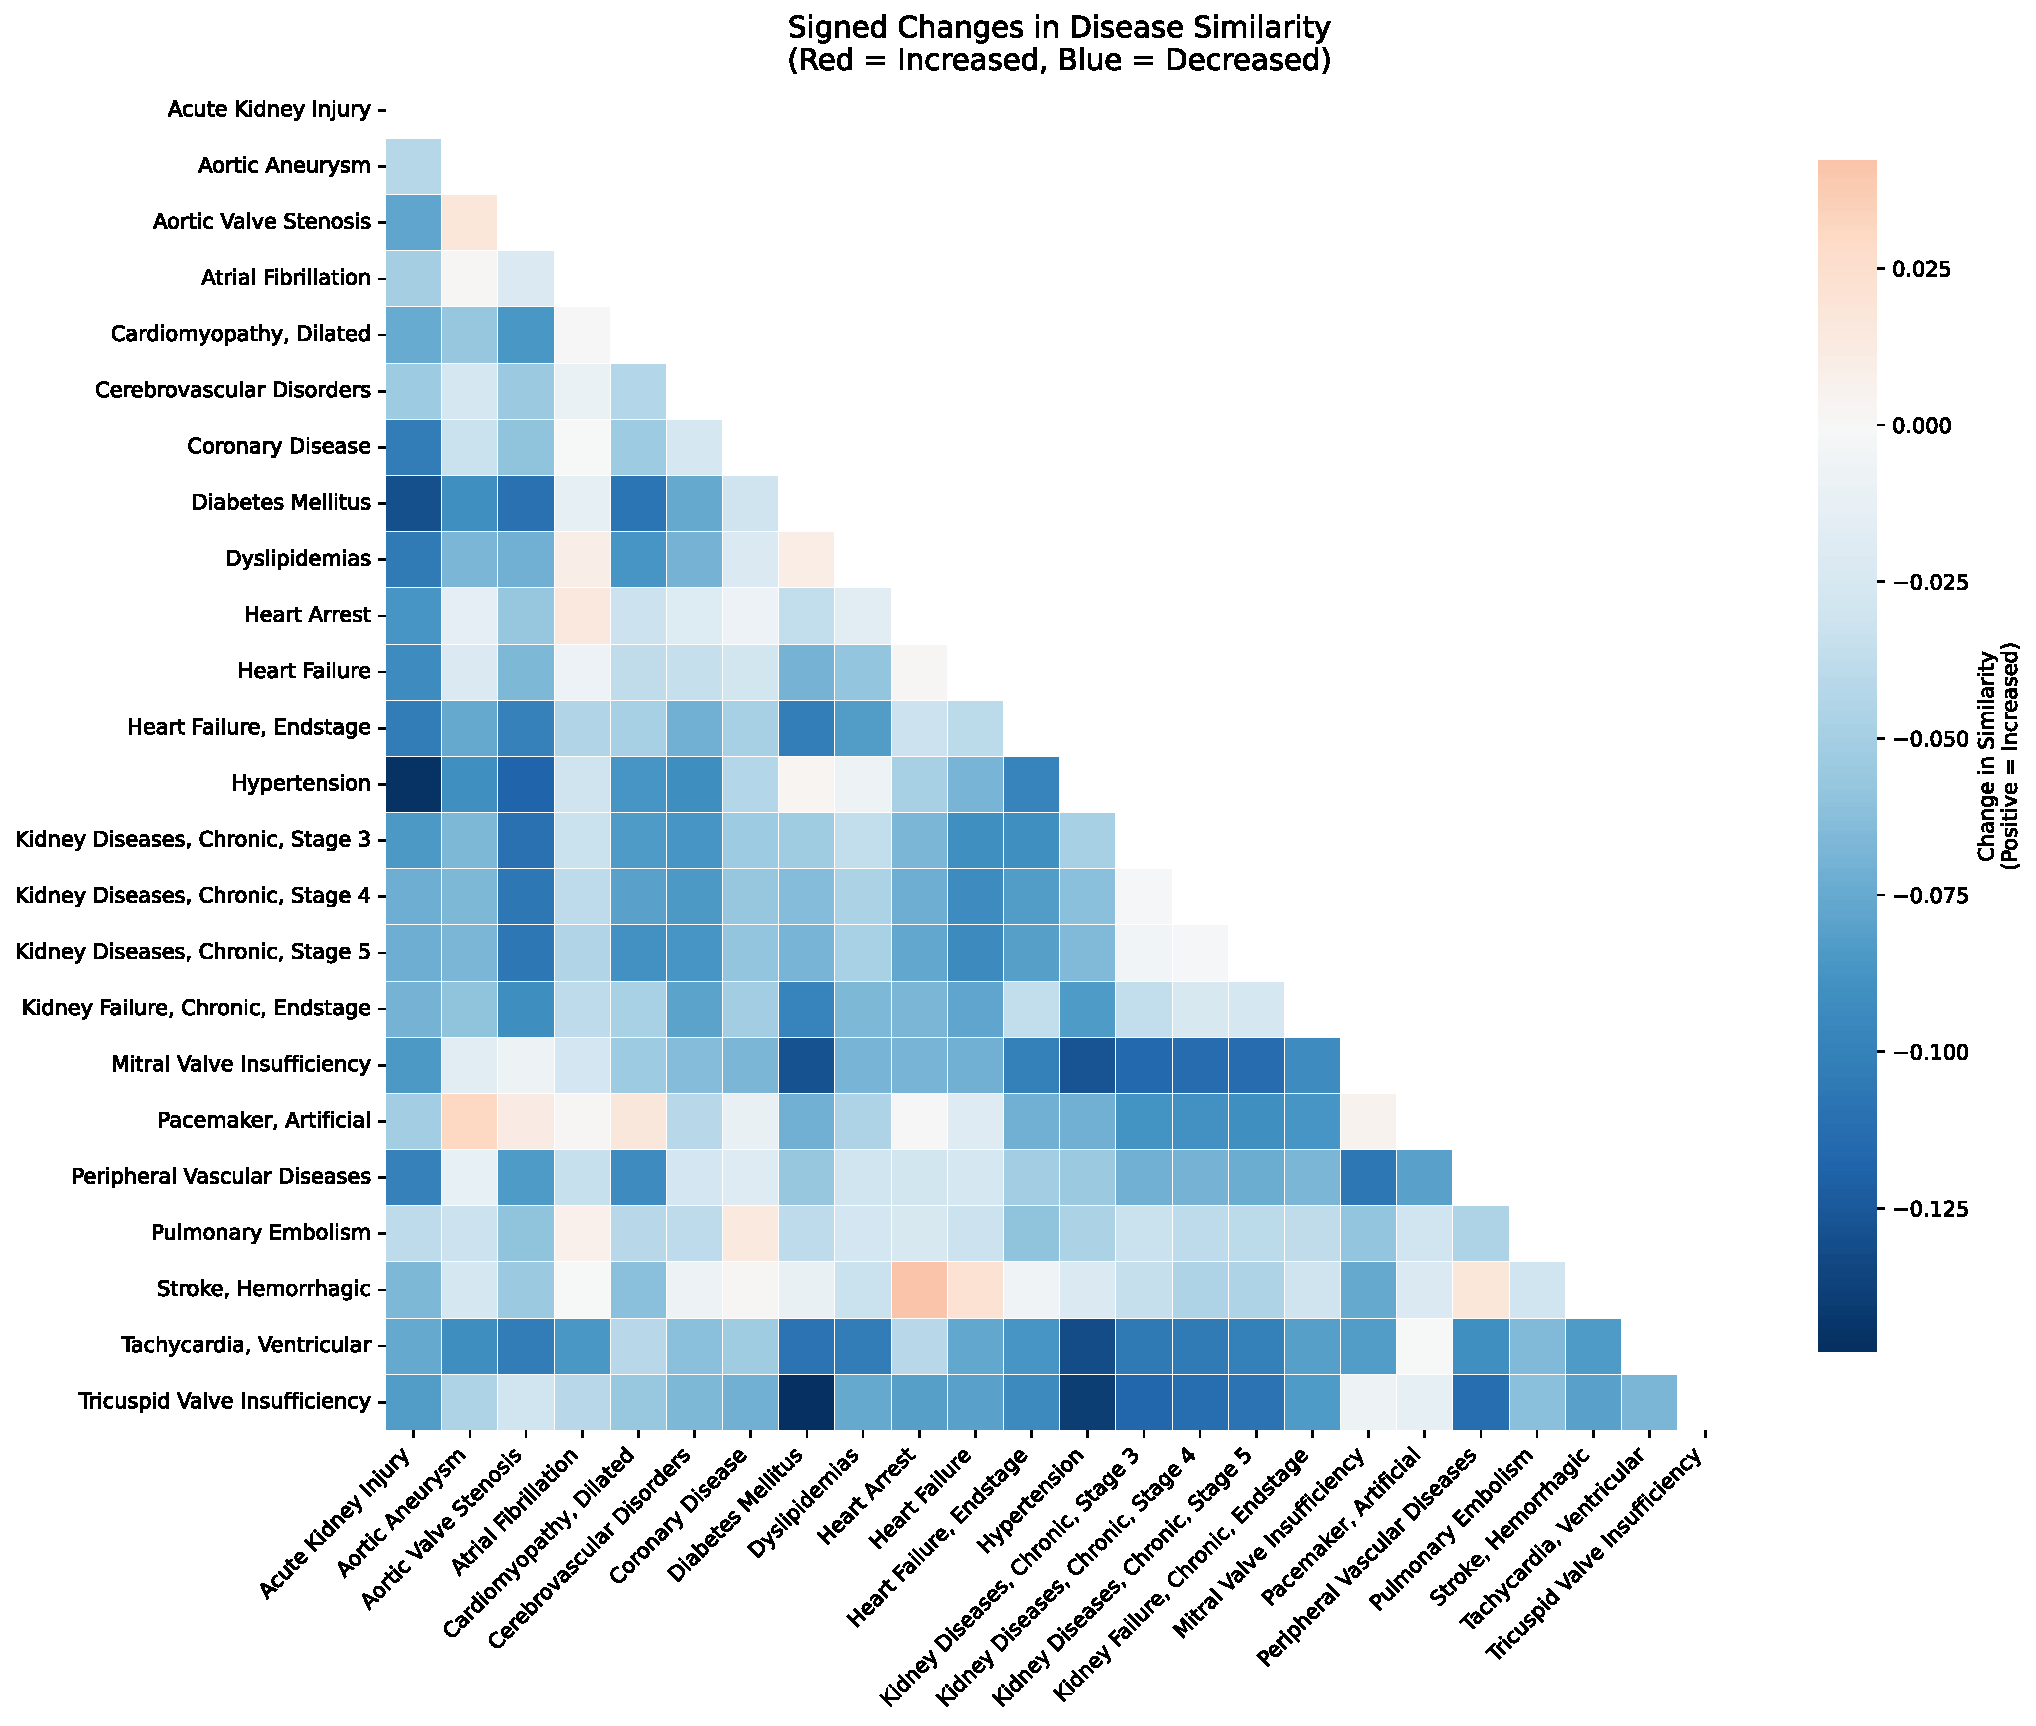
\includegraphics[width=0.9\textwidth]{Figures/disease_similarity_changes_signed.pdf}
    \caption{Signed changes in disease similarity after risk factor adjustment ($\Delta$). Blue indicates decreased similarity (confounding removal), red indicates increased similarity (unmasking true relationships).}
    \label{fig:disease_similarity_changes_signed}
\end{figure}
Global network comparison metrics are summarized in Table~\ref{tab:matrix_level_stats}. 252 of 276 disease pairs (91.3\%) exhibit decreased similarity after risk adjustment ($\Delta_{ij} < 0$), consistent with confounding removal. Only 24 pairs (8.7\%) show increased similarity ($\Delta_{ij} > 0$), potentially indicating relationships obscured by noise in the unadjusted network. The MAD across all disease pairs was moderate and the strongly negative MDC demonstrates a decreasing tendency in similarity after risk adjustment. The highly significant Wilcoxon test provides formal statistical evidence that these changes are systematic, confirming our hypothesis that shared risk factors artificially inflate disease similarities in the unadjusted network. The distribution of impact showed that 91.3\% of disease pairs experienced changes exceeding 1\%, with 12\% showing substantial changes above 10\%. Despite this evidence, Spearman correlation indicates that the fundamental ordering of disease relationships is largely preserved, suggesting that risk adjustment refines rather than fundamentally restructures the network. 

\begin{table}[h]
\centering
\begin{tabular}{lc}
\hline
\textbf{Metric} & \textbf{Value} \\
\hline
Mean Absolute Difference (MAD) & 0.060 \\
Mean Directional Change (MDC) & $-0.057$ \\
Wilcoxon signed-rank test & $p = 1.76 \times 10^{-44}$ \\
Spearman rank correlation & $\rho_S = 0.80$, $p = 3.80 \times 10^{-63}$ \\
\hline
\multicolumn{2}{l}{Impact distribution across disease pairs:} \\
\text{ } Pairs with change $> 1\%$ & 252 / 276 (91.3\%) \\
\text{ } Pairs with change $> 5\%$ & 159 / 276 (57.6\%) \\
\text{ } Pairs with change $> 10\%$ & 33 / 276 (12.0\%) \\
\hline
\end{tabular}
\caption{Matrix-level statistics comparing disease-only ($A^{(\mathcal{D})}$) versus risk-adjusted ($A^{(\mathcal{D+R})}$) similarity networks. MAD quantifies the average magnitude of change; MDC indicates systematic direction; Wilcoxon test evaluates the statistical significance of systematic change; Spearman correlation assesses structural preservation.}
\label{tab:matrix_level_stats}
\end{table}
Table~\ref{tab:top_affected_pairs_shared} reports the highly affected disease pairs (Section~\ref{subsub:conf_det} - Step 1) with the largest changes in similarity (top 5\%). All of these pairs showed a decrease in similarity. Hypertension and diabetes mellitus appear in 80\% of these most-affected pairs, particularly in association with valvular disorders and renal dysfunction. Conversely, advanced surgical interventions such as heart transplantation and artificial pacemaker implantation did not rank among the top-affected pairs, showing high stability across adjusted and unadjusted networks. To validate that these changes reflect confounding removal, we quantified shared risk factors for the most affected disease pairs (Section~\ref{subsub:conf_det} - Step 2 and 3). Highly affected disease pairs shared substantially more risk factors than lower-changed pairs (Mann-Whitney U test p-value = $2.57 \times 10^{-14}$), confirming that observed similarity decreases result from successful confounding removal rather than random variation.

\begin{table}[h]
\centering
\small
\begin{tabular}{cccc}
\hline
\textbf{Rank} & \textbf{Disease pair} & \textbf{Change} & \textbf{SharedRF} \\
\hline
1 & Tricuspid Valve Insufficiency $\leftrightarrow$ Diabetes Mellitus & -0.148 & 0.93 \\
2 & Acute Kidney Injury $\leftrightarrow$ Hypertension & -0.145 & 0.82 \\
3 & Tricuspid Valve Insufficiency $\leftrightarrow$ Hypertension & -0.140 & 0.91 \\
4 & Ventricular Tachycardia $\leftrightarrow$ Hypertension & -0.132 & 0.48 \\
5 & Acute Kidney Injury $\leftrightarrow$ Diabetes Mellitus & -0.130 & 0.86 \\
6 & Mitral Valve Insufficiency $\leftrightarrow$ Diabetes Mellitus & -0.129 & 0.83 \\
7 & Mitral Valve Insufficiency $\leftrightarrow$ Hypertension & -0.128 & 0.64 \\
8 & Hypertension $\leftrightarrow$ Aortic Valve Stenosis & -0.118 & 0.88 \\
9 & Tricuspid Valve Insufficiency $\leftrightarrow$ CKD Stage 3 & -0.117 & 0.98 \\
10 & Mitral Valve Insufficiency $\leftrightarrow$ CKD Stage 3 & -0.117 & 1.00 \\
11 & Mitral Valve Insufficiency $\leftrightarrow$ CKD Stage 4 & -0.114 & 1.00 \\
12 & Mitral Valve Insufficiency $\leftrightarrow$ CKD Stage 5 & -0.113 & 1.00 \\
13 & CKD Stage 4 $\leftrightarrow$ Tricuspid Valve Insufficiency & -0.112 & 0.99 \\
14 & Peripheral Vascular Diseases $\leftrightarrow$ Tricuspid Valve Insufficiency & -0.112 & 0.97 \\
\hline
\end{tabular}
\caption{Highly affected disease pairs (95-$th$ percentile), showing changes in similarity and SharedRF indicating the proportion of risk factors simultaneously associated (above threshold $\tau = 0.73$) with both diseases.}
\label{tab:top_affected_pairs_shared}
\end{table}

To assess the robustness of our confounding detection framework, we performed a sensitivity analysis by varying the risk factor definition threshold, $\tau$, across a range from $0.5$ to $0.9$. The results, documented in Supplementary Table~\ref{ST:shared_rf_sensitivity}, confirm the expected monotonic relationship: as $\tau$ increases, the number of risk factors associated with each disease and consequently the number of shared risk factors, decreases. At the upper bound ($\tau = 0.9$), the number of risk factors for each disease approaches zero, as this threshold significantly exceeds the mean similarity density of the risk factors' embeddings. The median achieves a balance between inclusion and exclusion of potential confounders. Notably, even as the number of individual risk factors per disease declines with higher $\tau$ values, the significance of the Mann-Whitney U test remains stable. This consistency demonstrates that our findings regarding confounding removal are robust to threshold specification. 

\subsection{Network sparsification and topology}\label{subsubsection:topology}
The sparse risk-adjusted cardiometabolic disease network, constructed using Gaussian Graphical Models, is shown as a binary adjacency matrix in Figure~\ref{fig:GGM_comorb_network_heatmap} with the corresponding graph visualization provided in Supplementary Figure~\ref{supp_mat:SF3}. Compared to the fully connected cosine similarity network, the GGM network exhibits only half of the edge density but the majority of pathophysiological relationships identified in Section~\ref{subsubsection:res_cosine}.
\begin{figure}[h]
    \centering
    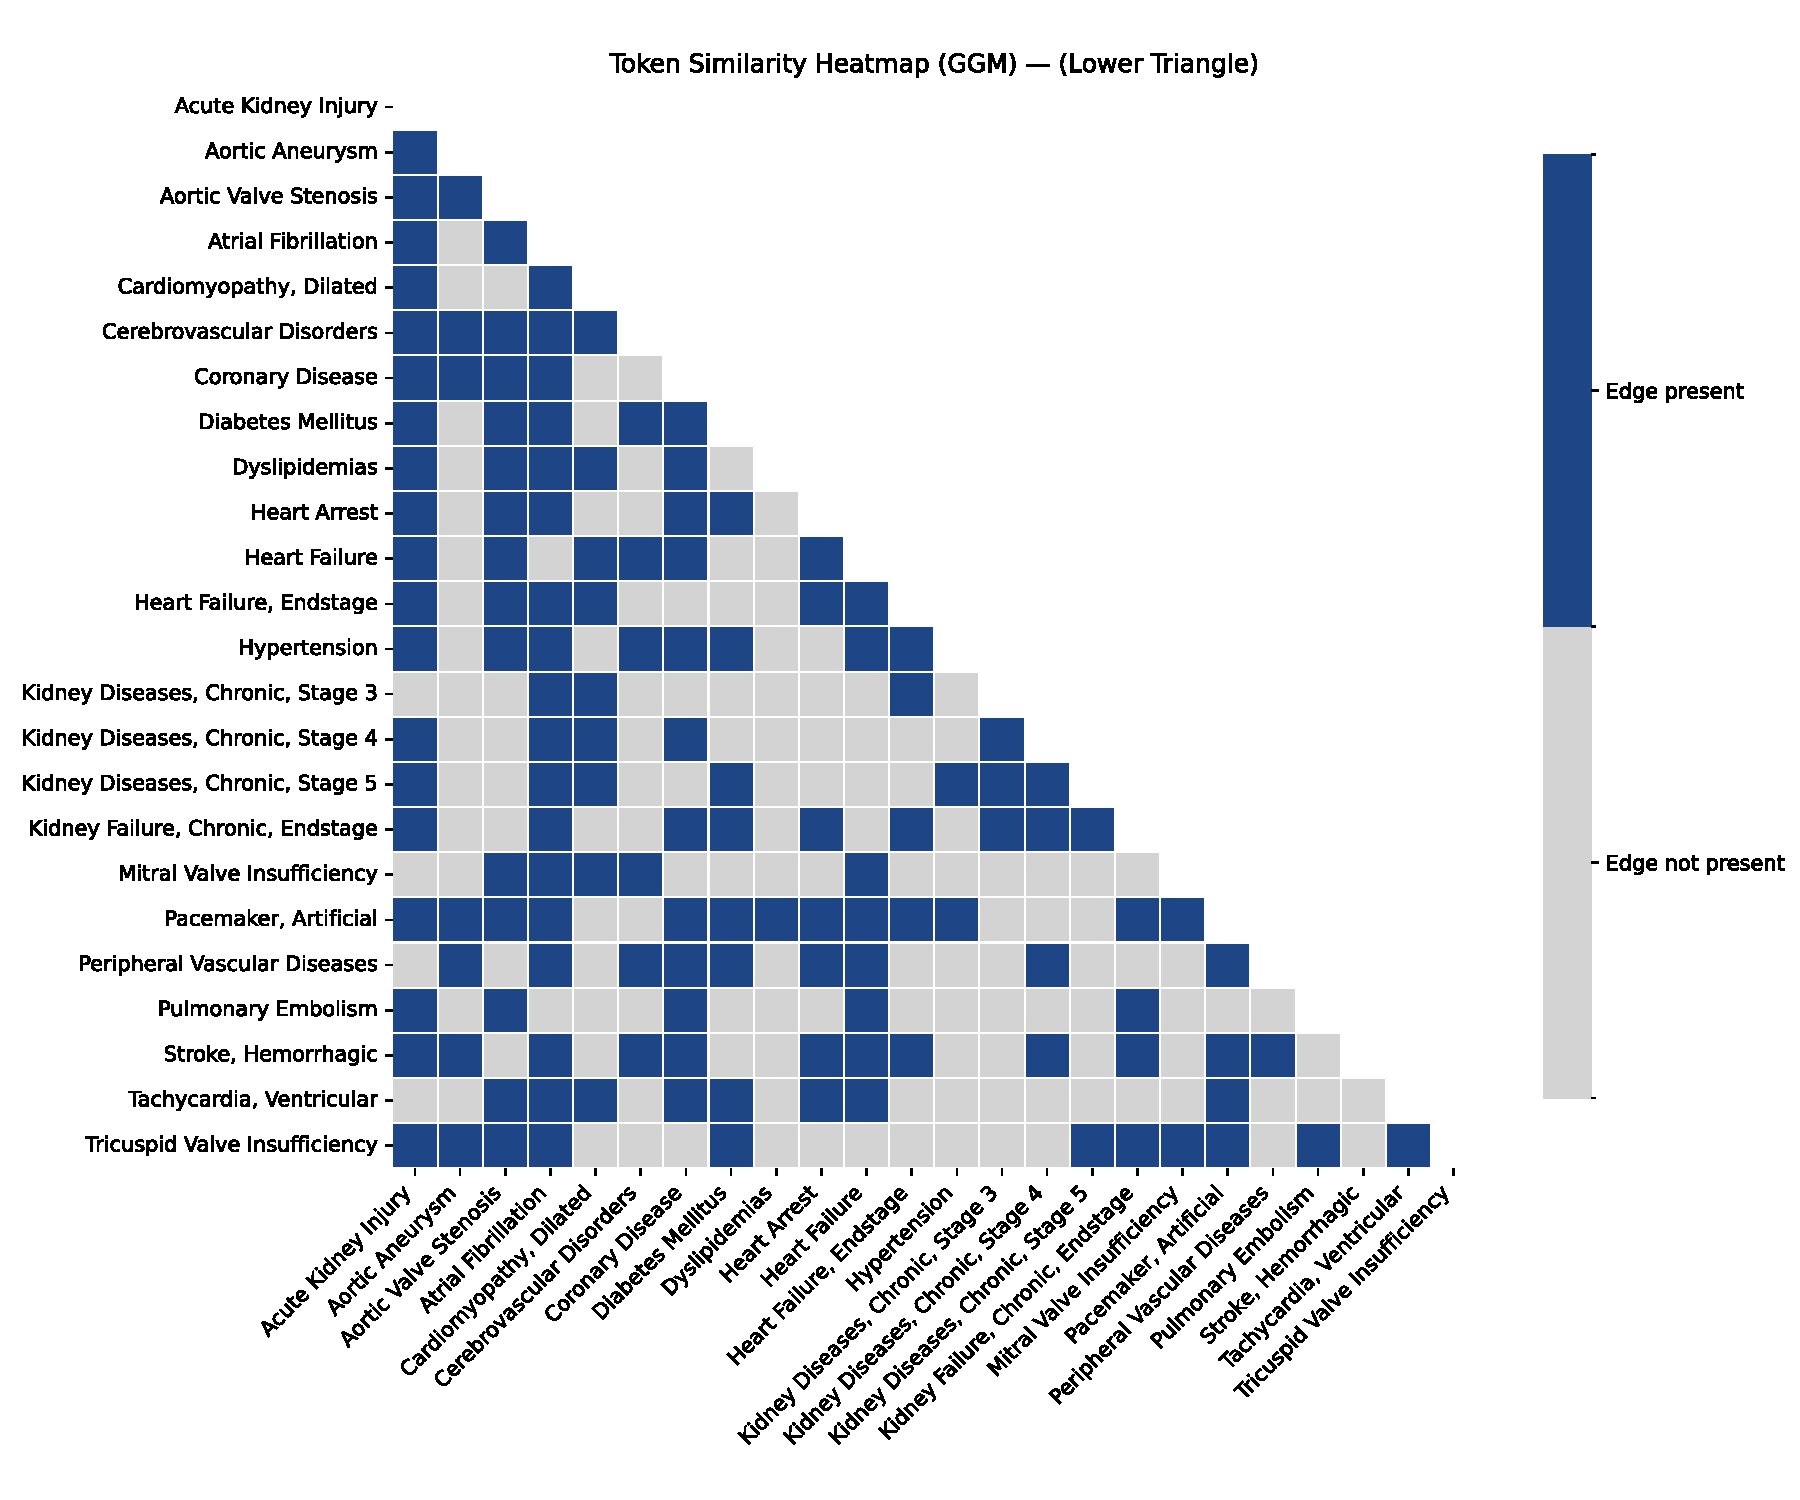
\includegraphics[width=0.9\textwidth]{Figures/disease_GGM_heatmap_main_par_binary.pdf}
    \caption{Cardiometabolic disease matrix estimated via Gaussian Graphical Lasso Regression computed from embeddings including both cardiometabolic diseases and risk factors. The graph representation is provided in Supplementary Figure~\ref{supp_mat:SF3}.}
    \label{fig:GGM_comorb_network_heatmap}
\end{figure}
To identify key pathological determinants within the network, we quantified node importance through degree and betweenness centrality measures. The results for the most central nodes are summarized in Table~\ref{tab:top5_centrality}, with comprehensive metrics for all phenotypes provided in Supplementary Table~\ref{ST:centrality}. Atrial fibrillation emerges as the primary hub with the highest degree and betweenness centrality, reflecting both its epidemiological prevalence and its critical position bridging multiple pathophysiological domains, including thromboembolism, heart failure, and cerebrovascular disease. Acute kidney injury ranks second in both centrality measures, underscoring its role as a key mediator within the cardiorenal syndrome pathway. The high betweenness centrality indicates that acute kidney injury facilitates the transition from acute cardiovascular insults to chronic renal dysfunction, connecting distinct pathological states. The elevated betweenness of the artificial pacemaker node, despite representing an intervention rather than a disease, reflects its function as a bridging state between primary arrhythmias, structural heart disease, and heart failure. Coronary disease occupies a central tier, linking ischemic pathophysiology to systemic metabolic disorders such as diabetes and peripheral vascular disease. While heart failure exhibits concentrated associations within cardiovascular and cardiorenal modules, the strong betweenness of aortic valve stenosis highlights its role in connecting valvular pathology to large-vessel disease. 

\begin{table}[h]
\centering
\small
\begin{tabular}{ccc}
\hline
\textbf{Rank} &\textbf{Degree} & \textbf{Betweeness} \\
\hline
1 & Atrial Fibrillation & Atrial Fibrillation \\
2 & Acute Kidney Injury & Acute Kidney Injury \\
3 & Artificial Pacemaker & Artificial Pacemaker \\
4 & Aortic Valve Stenosis / Coronary Disease & Coronary Disease \\
5 & Heart Failure & Aortic Valve Stenosis \\
\hline
\end{tabular}
\caption{Top 5 diseases ranked by betweenness and degree centrality in the GGM network. Details on centrality for other disease are provided in Supplementary Table~\ref{ST:centrality}.}
\label{tab:top5_centrality}
\end{table}

The application of the fast greedy modularity optimization algorithm to the GGM-derived network identified a latent community structure consisting of three distinct disease modules. This partition, shown in Figure~\ref{fig:community_detection}, reflects the primary biological domains of cardiometabolic pathology. The first module (cardiorenal-metabolic, color-coded blue) captures the continuum of heart-kidney failure, integrating progressive renal dysfunction with metabolic disorders. The second module (primary cardiovascular, color-coded pink) aggregates conditions originating from cardiac structural damage and electrical dysfunction. The third module (large vessel and cerebrovascular, color-coded green) shares the etiology of systemic vasculopathy, linking aortic pathology with peripheral and cerebral vascular disease. Notably, nodes such as acute kidney injury and atrial fibrillation were identified as inter-community bridges, maintaining high betweenness centrality while connecting the cardiorenal-metabolic and primary cardiovascular clusters.
 
\begin{figure}[h]
    \centering
    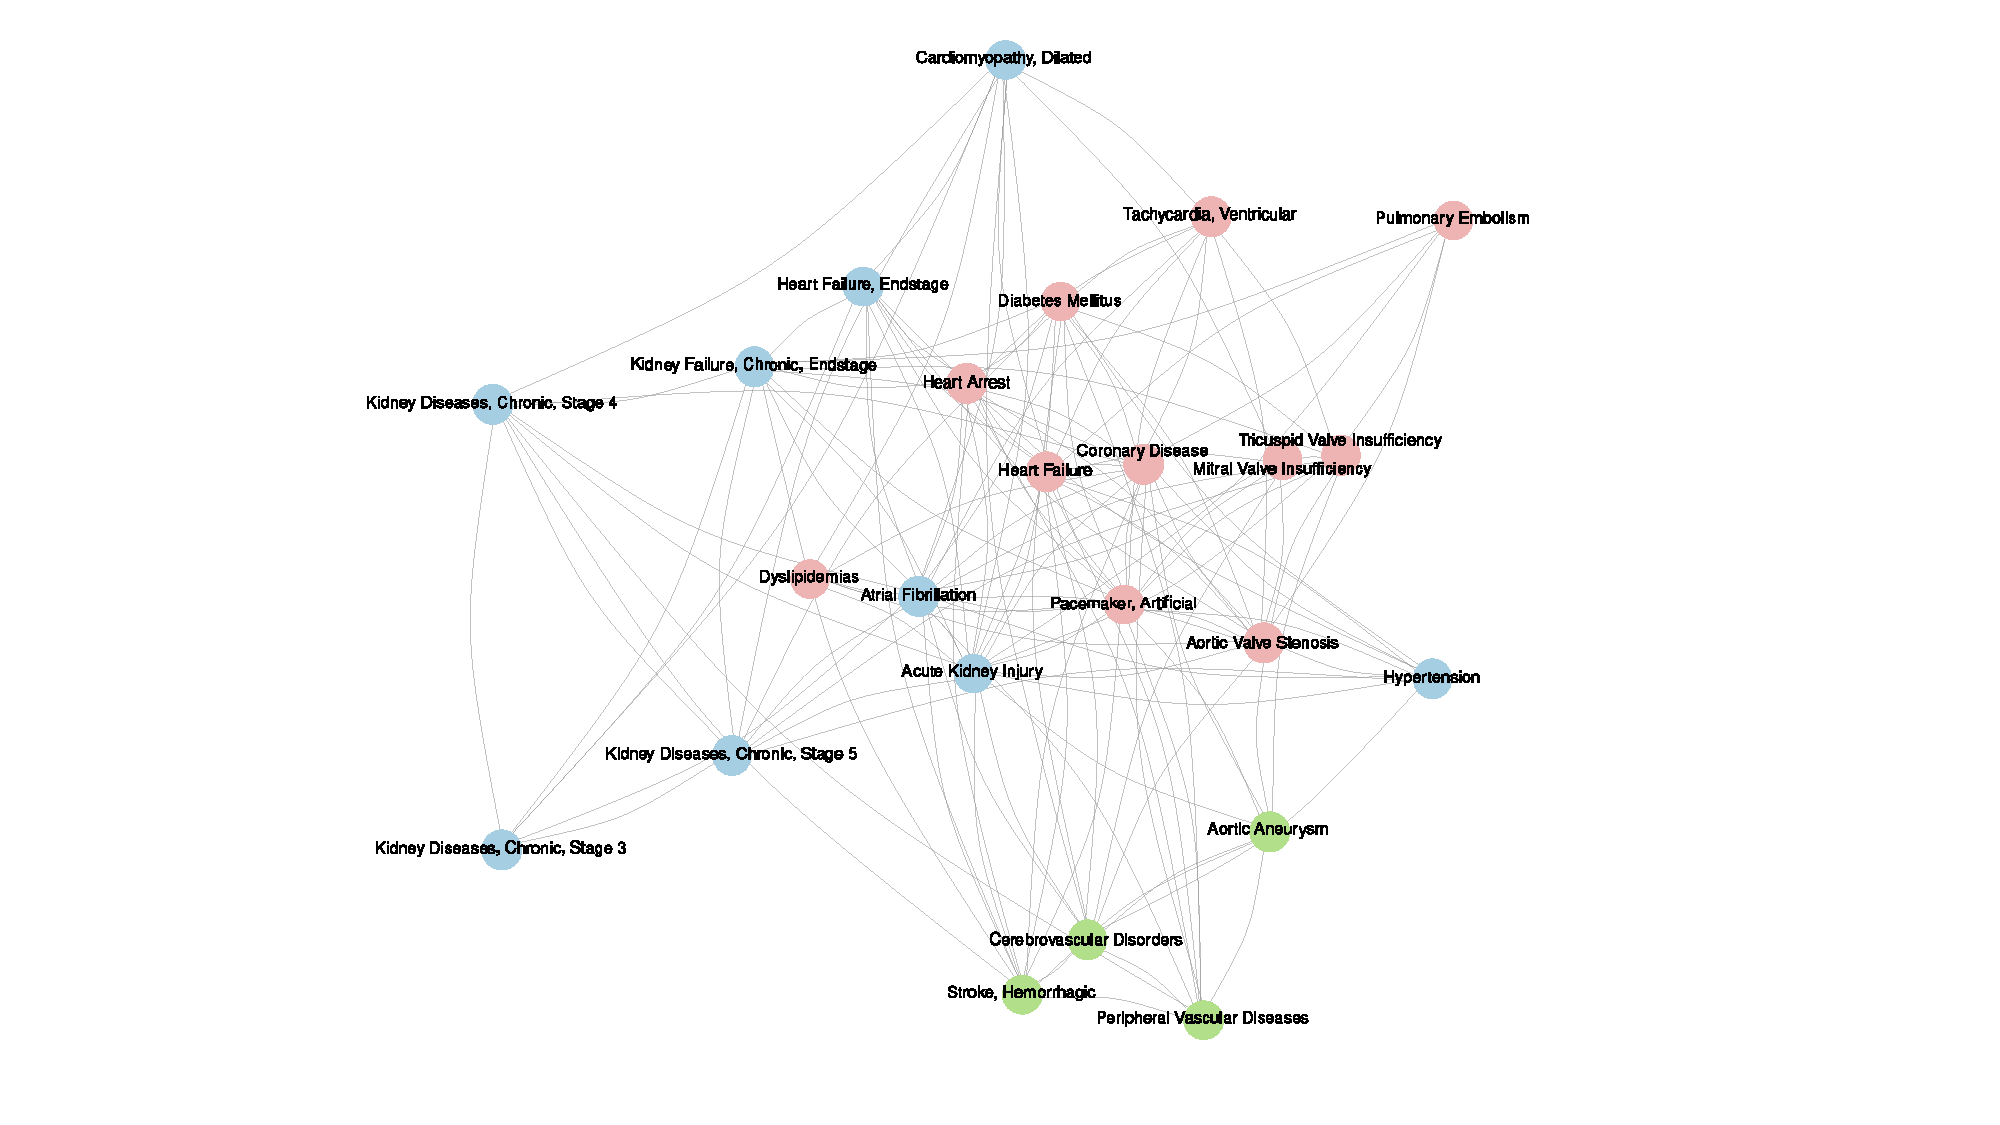
\includegraphics[width=0.95\textwidth]{Figures/community_detected.pdf}
    \caption{Community structure of the cardiometabolic disease network identified via fast greedy modularity optimization. Node colors indicate community membership: \textit{blue} = cardiorenal-metabolic module, \textit{pink} = primary cardiovascular module, \textit{green} = large vessel and cerebrovascular module.}
    \label{fig:community_detection}
\end{figure}



\section{Discussion}\label{sec:discussion}
Comorbidity networks provide a powerful framework for understanding disease relationships beyond simple co-occurrence statistics, revealing shared physiological mechanisms and guiding clinical management of multimorbidity. Understanding multimorbidity patterns is essential for developing effective, integrated, and person-centered care models~\cite{Chiadi2023}. A crucial advancement lies in analyzing disease combinations that exceed what would be expected by chance, addressing the high variability in how diseases co-occur, moving beyond simple prevalence rates and introducing patient-specific characteristics as risk factors ~\cite{EPF2012ChronicDiseaseResponse}. This shift is particularly important because knowledge of multimorbidity patterns has direct implications for patient-oriented (rather than disease-oriented) prevention, diagnosis, treatment, and prognosis, and, as highlighted by the National Institute for Health and Clinical Excellence, provides essential information for developing clinical guidelines and decision-support tools for managing patients with multiple chronic conditions~\cite{NICE2016NG56}. The integration of temporal information from longitudinal patient sequences represents a critical methodological advancement in this direction. By capturing both the dynamics and temporal ordering of disease progression, sequence-based methods can distinguish between early- and late-emerging conditions in the multimorbidity trajectory and identify the order in which diseases develop. Incorporating this temporal information allows for the construction of a more “realistic” comorbidity network, improving our understanding of the relationships between co-occurring diseases and informing the design of targeted intervention strategies~\cite{siggaard2020disease}. 

We developed a comprehensive methodological pipeline for constructing disease comorbidity from longitudinal patient data designed to overcome three key limitations of existing comorbidity network approaches: the absence of temporal information, confounding, and reliance on arbitrary thresholding for sparsification. Our approach adapts Word2Vec embeddings to learn disease representations from longitudinal patient trajectories, treating diseases as "words" and patient sequences as "sentences". This embedding-based framework offers several advantages over traditional co-occurrence statistics: dense 200-dimensional vectors capture richer information than scalar similarity measures, encoding both semantic relationships and temporal context; the continuous embedding space enables gradient-based optimization and transfer learning from large biomedical corpora; and incorporating risk factors allows shared patterns to be represented directly in the vector space, improving similarity estimates by reducing spurious associations driven by common exposures. Building on this principle, we introduce a confounding adjustment framework by jointly embedding diseases and risk factors. The model redistributes association signals: correlations driven by shared risk factors are allocated to risk factor dimensions, yielding adjusted disease embeddings that better reflect direct pathophysiological relationships. The difference between risk-adjusted and unadjusted similarities provides an interpretable measure of confounding magnitude for each disease pair, validated through a three-step framework demonstrating that observed decreases reflect genuine confounding removal rather than random variation. While we cannot definitively establish causality, the systematic correlation between similarity changes and shared risk factors provides strong evidence that our adjustment procedure successfully removes confounding. Applied to UK Biobank data with 24 cardiometabolic diseases and 76 risk factors, our framework revealed substantial confounding effects: 91.3\% of disease pairs showed decreased similarity after risk adjustment, with highly affected pairs systematically sharing more risk factors. Hypertension and diabetes mellitus appeared in 80\% of most-affected pairs, confirming that their frequent co-occurrence in unadjusted networks is heavily driven by shared lifestyle factors and comorbidities. Conversely, acute clinical events (acute myocardial infarction, cardiac arrest) and advanced interventions (heart transplantation, pacemaker implantation) showed minimal changes, appropriately reflecting their nature as acute events or end-stage treatments less confounded by gradual risk factor accumulation. For network sparsification, Gaussian Graphical Models provided a statistically principled alternative to traditional backboning methods~\cite{serrano2009extracting}, which fail when similarity values are homogeneous. GGM naturally handles such cases by modeling the full covariance structure and identifying edges that remain significant after conditioning on the entire network. Topological analysis of the GGM-derived network identified atrial fibrillation, acute kidney injury, and coronary disease as hub diseases with critical bridging functions, while community detection recovered three clinically meaningful modules (cardiorenal-metabolic, primary cardiovascular, large vessel cerebrovascular) aligning with established cardiometabolic taxonomy~(\cite{Chiadi2023, WHO_CVDs_2025}).

Beyond methodological contributions, our framework enables several clinically relevant applications that advance evidence-based practice in multimorbidity management. First, the topology-based identification of hub diseases and bridging nodes provides actionable insights for prioritizing preventive interventions. Diseases with high betweenness centrality, such as atrial fibrillation and acute kidney injury, represent strategic targets where interventions may have broad systemic impact across multiple pathophysiological domains~\cite{Zhao2023ComorbidityNetwork}. Second, recent research has shown that comorbidity networks can evolve over time, with disease association patterns shifting across life stages and phases of progression~(\citealp{dervic2025comorbidity, gardinazzi2025characterization}). Our embedding-based framework can be readily extended to construct age-specific networks by applying the pipeline to stratified cohorts based on age. This reveal how multimorbidity patterns change over the life course and how the influence of risk factors varies with age. Methodologically, temporal differences can be identified in the same way we compared adjusted and unadjusted networks, by systematically contrasting networks constructed under different modeling specifications. Third, patient-specific representations create new opportunities for personalized risk stratification. By mapping individual patient trajectories into the learned embedding space, representing each patient as the mean embedding of the diseases recorded in their clinical history, we can cluster patients with similar comorbidity progression patterns. This enables stratified survival analyses and the identification of profiles that deviate from typical trajectories, thereby supporting earlier detection and intervention for high-risk multimorbidity phenotypes~\cite{liang2024comorbidity}.Fourth, multimorbidity patterns identified through our framework can serve as predictors of intense healthcare usage and adverse health outcomes. As demonstrated by~\cite{Wolff2002}, the simultaneous presentation of diseases may have multiplicative rather than additive effects on health and healthcare costs. Network-derived features, such as membership in high-risk disease modules or proximity to hub diseases, could enhance prediction models for disability, adverse drug events, and increased disease severity, ultimately supporting resource allocation and care planning decisions~\cite{buja2025healthcare}.

Our study has several limitations that suggest directions for methodological development. First, while we adjust for 76 measured risk factors, residual confounding from unmeasured variables may persist. Future work could enrich the set of information by integrating genetic, proteomic, and metabolomic data to reveal shared underlying biological mechanisms and identify potential therapeutic targets that extend across multiple conditions~\citep{Sibilio2025, nam2020network}. Second, the embedding approach assumes that diseases appearing in similar temporal contexts have similar meanings, which may not hold for all disease pairs. Rare diseases with few occurrences may be poorly represented in the embedding space, potentially missing important but uncommon comorbidity patterns. Additionally, diseases with multiple distinct etiologies (e.g., heart failure with preserved or reduced ejection fraction) are treated as single entities, potentially obscuring heterogeneity. Future extensions could incorporate disease subtypes when data availability and sufficient sample sizes permit. Third, while we capture temporal ordering at the disease level, we do not explicitly model time intervals between events or disease onset ages, which may contain prognostic information. In addition, the estimated similarity networks are undirected, precluding inference of disease progression directionality or causal pathways. Although temporal sequence information informs the embeddings, the resulting networks represent associations rather than directional dependencies. 
Incorporating causal inference frameworks~(\citealp{pearl2009causality, prosperi2020causal, xu2019patient, kong_causal}) could enable directed network estimation, distinguishing causes from effects in disease relationships and supporting the construction of age-dependent or temporally evolving networks that track disease progression trajectories over the life course.

In conclusion, this work demonstrates that integrating longitudinal patient data with explicit risk factor adjustment and advanced representation learning substantially enhances the validity and clinical utility of disease network analyses. By addressing key limitations in existing approaches our framework provides a statistically rigorous foundation for characterizing multimorbidity patterns. The systematic pipeline we present offers a generalizable strategy applicable beyond cardiometabolic conditions, with direct implications for evidence-based guideline development, patient stratification and healthcare resource planning. These applications link research with practice, paving the way for more precise characterization of multimorbidity patterns and their underlying mechanisms across diverse disease domains.


%%COMMENTI CLINICI RIMOSSI
%Highly affected disease pairs shared substantially more risk factors than lower-ranked pairs, with all 14 most-affected pairs showing decreased similarity after adjustment. Similarly, associations involving mitral and tricuspid valve insufficiency are highly confounded by shared hemodynamic risks such as hypotension, cardiac complications, and conduction disorders, inflating their apparent relationships with metabolic conditions in unadjusted networks. Collectively, our findings suggest that the network topology effectively recovers clinical progression pathways, identifying strategic nodes governing transitions between distinct pathological states. In particular, the dual prominence of atrial fibrillation highlights its high local connectivity and strategic bridging function, identifying it as a key mechanistic hub where interventions may have broad systemic impact. Community detection identified three disease modules, metabolic, primary cardiovascular, and large vessel cerebrovascular, aligning with established cardiometabolic disease taxonomy and demonstrating that our data-driven approach naturally recovers clinically meaningful disease groupings~(\citealp{Chiadi2023, WHO_CVDs_2025}).


%\section{Software}
%\label{sec5}
%Software in the form of R code, together with a sample input data set and complete documentation is available on request from the corresponding author (eaheron@tcd.ie).


%\section{Supplementary Material}
%\label{sec6}

%Supplementary material is available online at
% \href{http://biostatistics.oxfordjournals.org}%
% {http://biostatistics.oxfordjournals.org}.
%\url{http://biostatistics.oxfordjournals.org}.


\section*{Acknowledgments}
The present research has been supported by MUR, grant Dipartimento di Eccellenza 2023- 2027.
F. Ieva acknowledges the National Plan for NRRP Complementary Investments "Advanced Technologies for Human-centred Medicine" (PNC0000003). We also thank Carlo Andrea Pivato and Laura Savaré for their support in the phenotype definitions.
\\
{\it Conflict of Interest}: None declared.

\section*{Data sharing}
UKB data are accessible for health-related research in the public interest. This study used data from the UKB Resource under Application Number 102297.


\newpage
\section*{Supplementary Material}
\setcounter{table}{0}          
\renewcommand{\thetable}{S\arabic{table}}

\setcounter{subsection}{0}
\renewcommand{\thesubsection}{S\arabic{subsection}}

\subsection{Supplementary Method: traditional sparsification approaches}\label{supp_met_1}
\subsubsection{Backbone extraction via disparity filter}\label{subsec:backbone}
The disparity filter~\cite{serrano2009extracting} identifies statistically significant edges by comparing observed edge weights to a null model of uniform weight distribution. For each disease node $i$ with degree $k_i$ (considering all edges), the probability that edge weight $w_{ij}$ could arise by chance under uniform redistribution is:
\begin{equation}\label{eq:disparity_filter}
\alpha_{ij} = (1 - p_{ij})^{k_i - 1}
\end{equation}
where $p_{ij} = w_{ij} / s_i$ is the proportion of node $i$'s total weight $s_i = \sum_j w_{ij}$ allocated to edge $(i,j)$.

Edges with $\alpha_{ij} < \alpha_{\text{sig}}$ (typically $\alpha_{\text{sig}} = 0.05$) are retained, indicating their weights are significantly larger than expected under uniform redistribution. This produces a sparse "backbone" network preserving the most statistically salient relationships.

We apply the disparity filter to $A^{\mathcal{D+R}}$ at significance level $\alpha_{\text{sig}} = 0.05/n_{pairs}$, where $n_{pairs} = 2760$. This approach resulted in an empty network, even when the significance level was increased to $\alpha_{\text{sig}} = 0.05$. 

\subsubsection{Locally adapted network sparsification}\label{subsec:lans}
The Locally Adapted Network Sparsification (LANS) method~\cite{marcaccioli2022locally} addresses limitations of global thresholding by adapting significance thresholds to local network topology. Building on the noise-corrected backbone extraction framework~\cite{foti2011nonparametric}, LANS estimates a node-specific null model that accounts for the local strength distribution of edges. For each node $i$, the method computes a local significance threshold based on the distribution of edge weights incident to that node. Specifically, for edge $(i,j)$ with weight $w_{ij}$, the local p-value is computed as:
\begin{equation}\label{eq:lans}
p_{ij}^{\text{local}} = P(W \geq w_{ij} | \mathcal{N}_i)
\end{equation}
where $\mathcal{N}_i$ denotes the neighborhood of node $i$ and the null distribution is estimated from the empirical distribution of weights in $\mathcal{N}_i$. Edges are retained if $p_{ij}^{\text{local}} < \alpha_{\text{sig}}$ for both nodes $i$ and $j$, ensuring that the edge is locally significant from both endpoints' perspectives. This adaptive approach is particularly effective for networks with heterogeneous degree distributions or highly variable edge weight patterns, as it avoids the assumption of a single global null model. Implementation was performed using the LANS R package~\cite{marcaccioli2022locally}. We applied LANS to the risk-adjusted similarity network $A^{(\mathcal{D}+\mathcal{R})}$ with significance level $\alpha_{\text{sig}} = 0.05/n_{pairs}$. However, this approach resulted in an extremely sparse network showed in Figure~\ref{SF:backboning} which retains only 10 edges (3.6\% retention rate), with several clinically central diseases, including diabetes mellitus, hypertension, and multiple valvular conditions, left isolated without any connections.

\setcounter{figure}{0}          
\renewcommand{\thefigure}{SM-F\arabic{figure}}

\begin{figure}[h!]
    \centering
    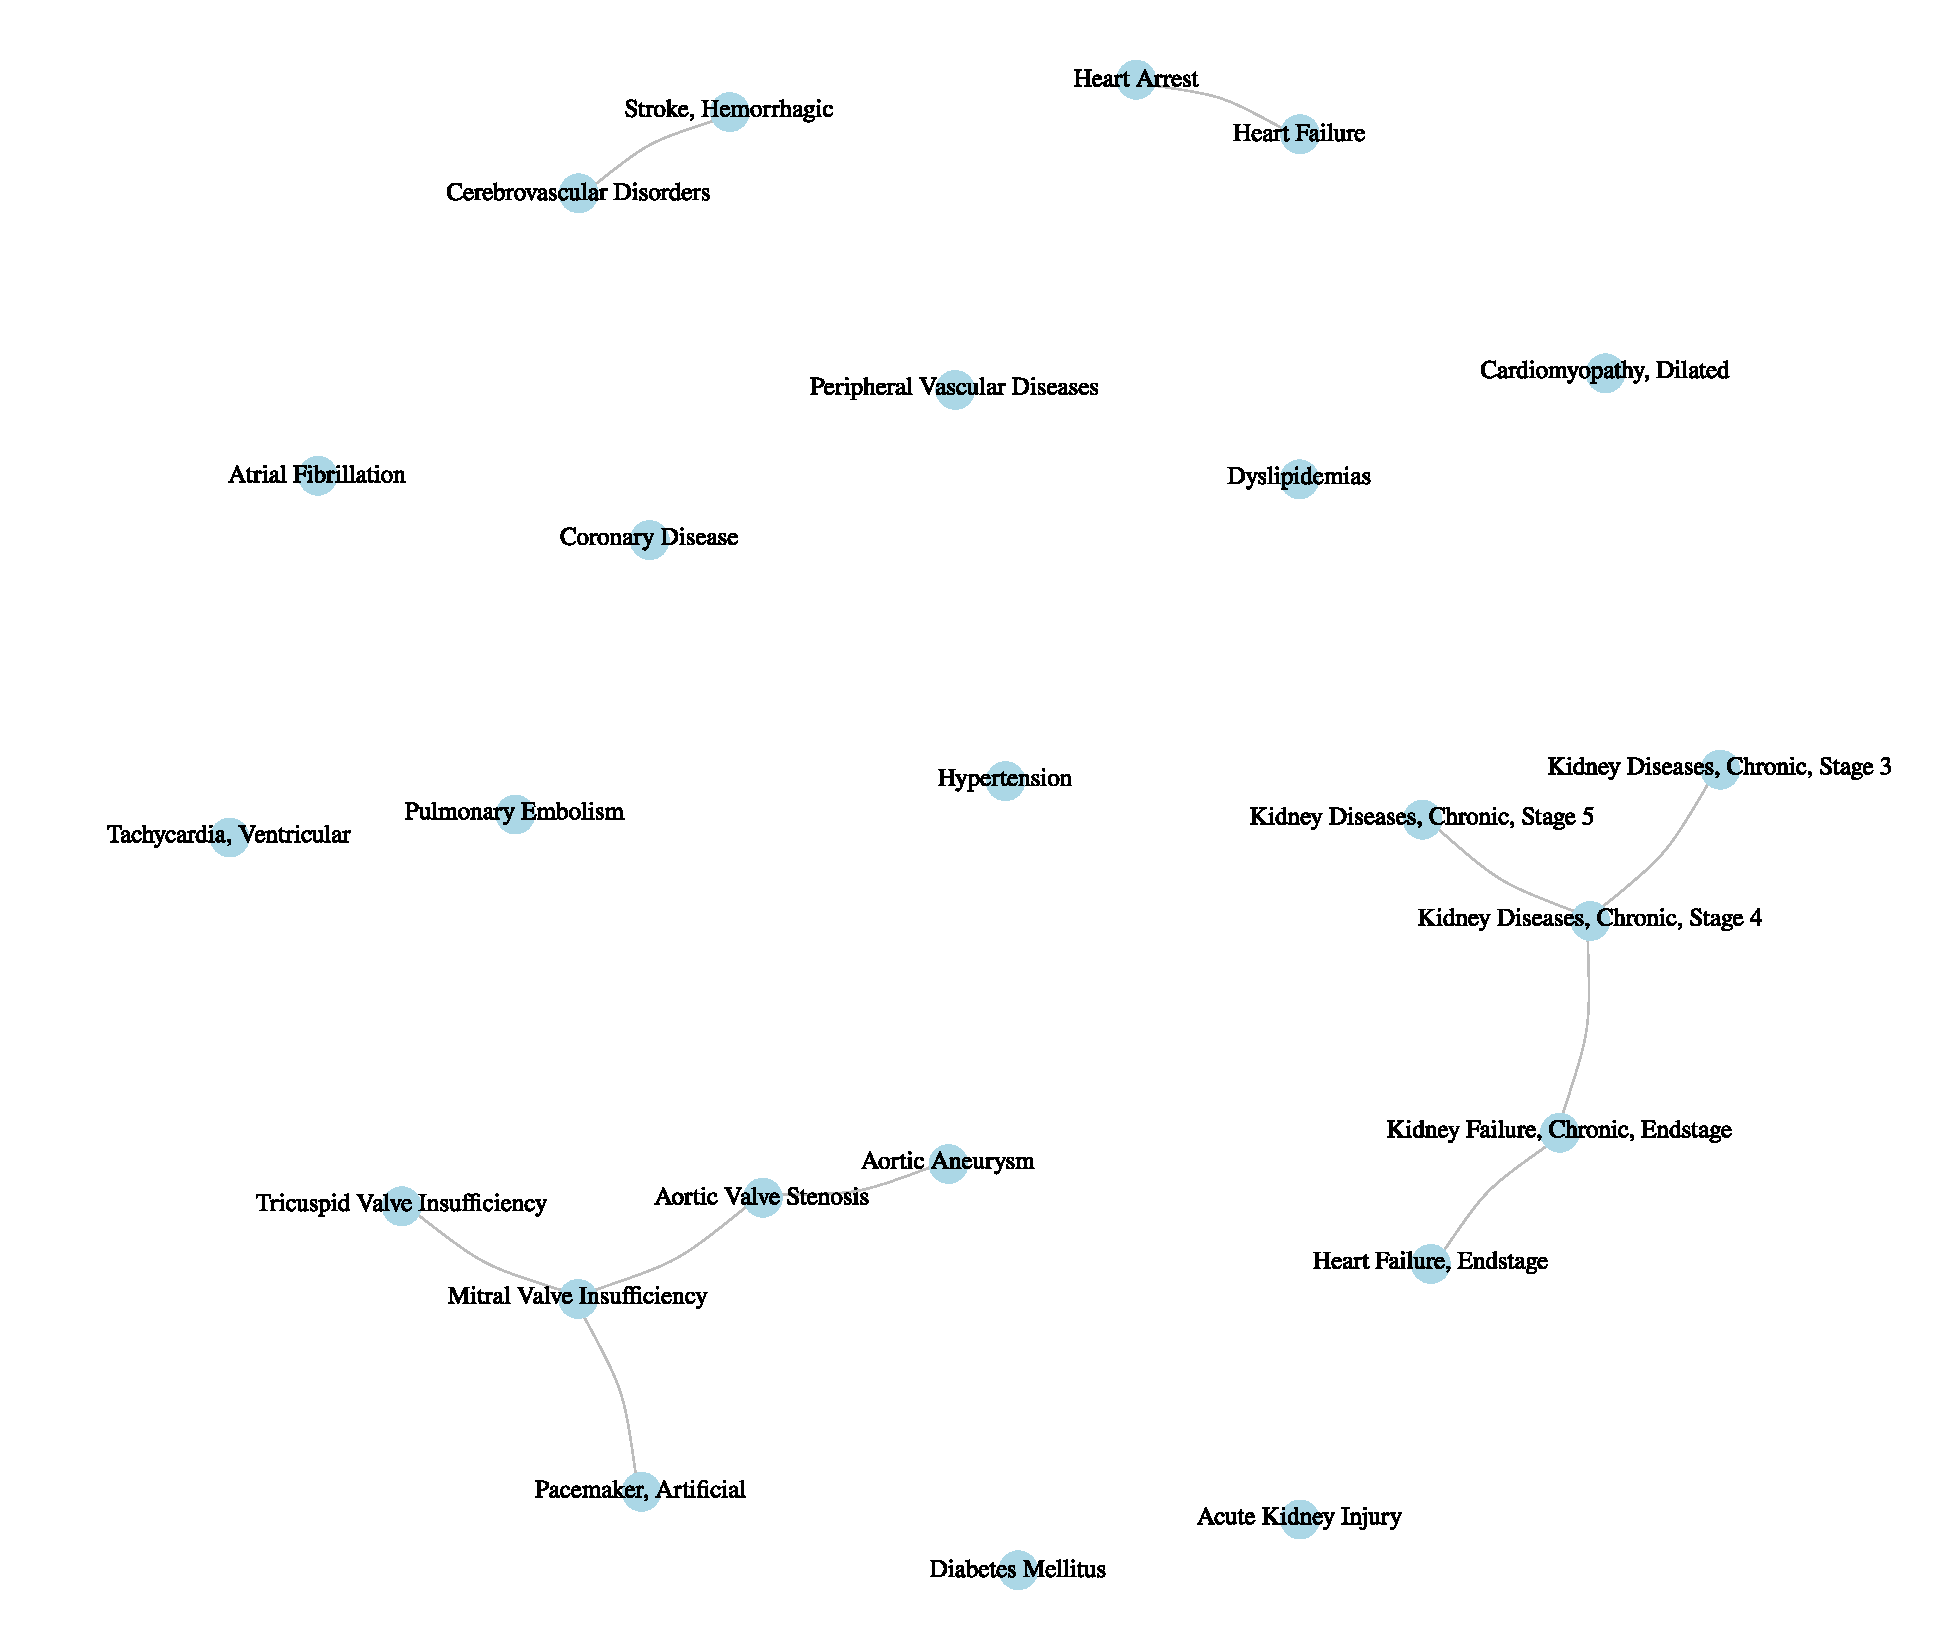
\includegraphics[width=1\textwidth]{Figures/Plots_backbone_main_par_comorb_diseases.pdf}
    \caption{Risk-adjusted Cardiometabolic disease network estimated via Locally adapted network sparsification.}
    \label{SF:backboning}
\end{figure}

This over-sparsification reflects a fundamental limitation of locally adaptive methods when applied to fully connected networks with relatively homogeneous, uniformly strong associations. In our similarity network, edge weights range narrowly (IQR range = 0.66-81, median = 0.74), with the majority of disease pairs exhibiting moderate-to-strong similarities. Under such conditions, local null models fail to distinguish genuine associations from background signal, as all edges appear locally significant or insignificant depending on arbitrary neighborhood definitions. The LANS method implicitly assumes substantial local heterogeneity in edge strengths, a condition not met in our embedding, based similarity network where diseases cluster into cohesive modules with consistently high internal similarities.

For these reasons, we concluded that statistically-based backboning methods are inadequate for sparsifying fully connected, homogeneously weighted similarity networks. This motivated our adoption of Gaussian Graphical Models (Section~\ref{subsec:sparsification}), which provide sparsification through conditional independence estimation rather than relying on assumptions about weight distribution heterogeneity.

\newpage
\subsection*{Supplementary Tables}
\begin{table}[h]
\centering
\caption{Cardiometabolic phenotypes definition with lifecourse incidence main diseases.}
\label{ST:table1}
\vspace{2mm}
\footnotesize Source: \url{https://htechnopole-my.sharepoint.com/:x:/r/personal/alessia_mapelli_fht_org/Documents/Dott/4th%20Year/SIS%202026/SIS_AM_NF_comorb_network/mapping_diseases.xlsx?d=we12a501ed7ec4cd49dea4ecebd599e85&csf=1&web=1&e=iBeF6F&nav=MTVfezY4RTgwMDg3LTNDRTUtNEM1OS1BM0RGLUJCNDgxRThFRDBDM30}
\end{table}

\begin{table}[h]
\centering
\caption{Risk factors phenotypes definition}
\label{ST:table2}
\vspace{2mm}
\footnotesize Source: \url{https://htechnopole-my.sharepoint.com/:x:/r/personal/alessia_mapelli_fht_org/Documents/Dott/4th%20Year/SIS%202026/SIS_AM_NF_comorb_network/mapping_diseases.xlsx?d=we12a501ed7ec4cd49dea4ecebd599e85&csf=1&web=1&e=XrGTiF&nav=MTVfezAwMDAwMDAwLTAwMDEtMDAwMC0wMDAwLTAwMDAwMDAwMDAwMH0}
\end{table}

\begin{table}[ht]
\centering
\caption{Shared risk factors for each disease pair across different sensitivity thresholds.}
\label{ST:shared_rf_sensitivity}
\small
\begin{tabular}{|l|c|c|c|c|c|c|}
\hline
\textbf{Disease Pair} & \textbf{0.5} & \textbf{0.6} & \textbf{0.7} & \textbf{0.72*} & \textbf{0.8} & \textbf{0.9} \\
\hline
TVI $\leftrightarrow$ DM   & 1.00 & 1.00 & 0.91 & \textbf{0.93} & 0.50 & 0.00 \\
AKI $\leftrightarrow$ HTN  & 1.00 & 0.99 & 0.91 & \textbf{0.82} & 0.50 & 0.00 \\
TVI $\leftrightarrow$ HTN  & 1.00 & 1.00 & 0.93 & \textbf{0.91} & 0.50 & 0.00 \\
VT $\leftrightarrow$ HTN   & 0.99 & 0.95 & 0.80 & \textbf{0.48} & 0.00 & 0.00 \\
AKI $\leftrightarrow$ DM   & 1.00 & 0.99 & 0.87 & \textbf{0.86} & 0.50 & 0.00 \\
MVI $\leftrightarrow$ DM   & 1.00 & 0.99 & 0.89 & \textbf{0.83} & 0.00 & 0.00 \\
MVI $\leftrightarrow$ HTN  & 1.00 & 0.95 & 0.78 & \textbf{0.64} & 0.00 & 0.00 \\
HTN $\leftrightarrow$ AVS  & 1.00 & 1.00 & 0.93 & \textbf{0.88} & 0.50 & 0.00 \\
TVI $\leftrightarrow$ CKD3 & 1.00 & 0.99 & 0.99 & \textbf{0.98} & 1.00 & 0.00 \\
MVI $\leftrightarrow$ CKD3 & 1.00 & 1.00 & 1.00 & \textbf{1.00} & 0.80 & 0.00 \\
MVI $\leftrightarrow$ CKD4 & 1.00 & 1.00 & 1.00 & \textbf{1.00} & 1.00 & 0.00 \\
MVI $\leftrightarrow$ CKD5 & 1.00 & 1.00 & 1.00 & \textbf{1.00} & 0.80 & 0.00 \\
CKD4 $\leftrightarrow$ TVI & 1.00 & 1.00 & 0.99 & \textbf{0.99} & 0.87 & 0.25 \\
PVD $\leftrightarrow$ TVI  & 1.00 & 0.97 & 0.97 & \textbf{0.97} & 0.96 & 0.00 \\
\hline
\textbf{Mean (SD)} & 0.99 (0.002) & 0.98 (0.02) & 0.93 (0.07) & \textbf{0.88 (0.15)} & 0.57 (0.36) & 0.02 (0.07) \\
\textbf{MW test p-value} & $8.51 \times 10^{-15}$ & $5.24 \times 10^{-15}$ & $6.43 \times 10^{-14}$ & $\mathbf{2.57 \times 10^{-14}}$ & $9.67 \times 10^{-11}$ & NA \\
\hline
\end{tabular}
\vspace{0.8em}
\footnotesize
\vspace{0.3em}
\footnotesize
\parbox{0.97\linewidth}{
\textit{Note:} Abbreviations: TVI = Tricuspid Valve Insufficiency, MVI = Mitral Valve Insufficiency, DM = Diabetes Mellitus, HTN = Hypertension, AKI = Acute Kidney Injury, VT = Ventricular Tachycardia, AVS = Aortic Valve Stenosis, CKD3-5 = Chronic Kidney Disease stages 3-5, PVD = Peripheral Vascular Diseases. *Main analysis threshold. MW test = Mann-Whitney U test\\
For $\tau = 0.9$ the Mann-Whitney U test was not applicable due to the high number of zeros.
}
\end{table}

\newpage

\begin{table}[h]
\centering
\begin{tabular}{lcc}
\hline
\textbf{Disease} & \textbf{Degree Centrality} & \textbf{Between Centrality} \\
\hline
Atrial Fibrillation & 1 & 1 \\
Acute Kidney Injury & 2 & 2 \\
Artificial Pacemaker & 3 & 3 \\
Coronary Disease & 4 & 4 \\
Aortic Valve Stenosis & 4 & 5 \\
Heart Failure & 6 & 6 \\
Dilated Cardiomyopathy & 11 & 7 \\
Chronic Kidney Failure Endstage & 7 & 8 \\
Tricuspid Valve Insufficiency & 11 & 9 \\
Diabetes Mellitus & 7 & 10 \\
Heart Failure, Endstage & 11 & 11 \\
Cerebrovascular Disorders & 11 & 12 \\
Stroke, Hemorrhagic & 9 & 13 \\
Chronic Kidney Diseases, Stage 4 & 17 & 14 \\
Chronic Kidney Diseases, Stage 5 & 17 & 15 \\
Peripheral Vascular Diseases & 15 & 16 \\
Heart Arrest & 9 & 17 \\
Hypertension & 15 & 18 \\
Tachycardia, Ventricular & 17 & 19 \\
Aortic Aneurysm & 20 & 20 \\
Mitral Valve Insufficiency & 21 & 21 \\
Pulmonary Embolism & 22 & 22 \\
Chronic Kidney Diseases, Stage 3 & 22 & 23 \\
Dyslipidemias & 22 & 24 \\
\hline
\end{tabular}
\caption{Centrality measures for diseases.}
\label{ST:centrality}
\end{table}

\setcounter{figure}{0}          
\renewcommand{\thefigure}{S\arabic{figure}}

\clearpage


\subsection*{Supplementary Figure}
\begin{figure}[H]
    \centering
    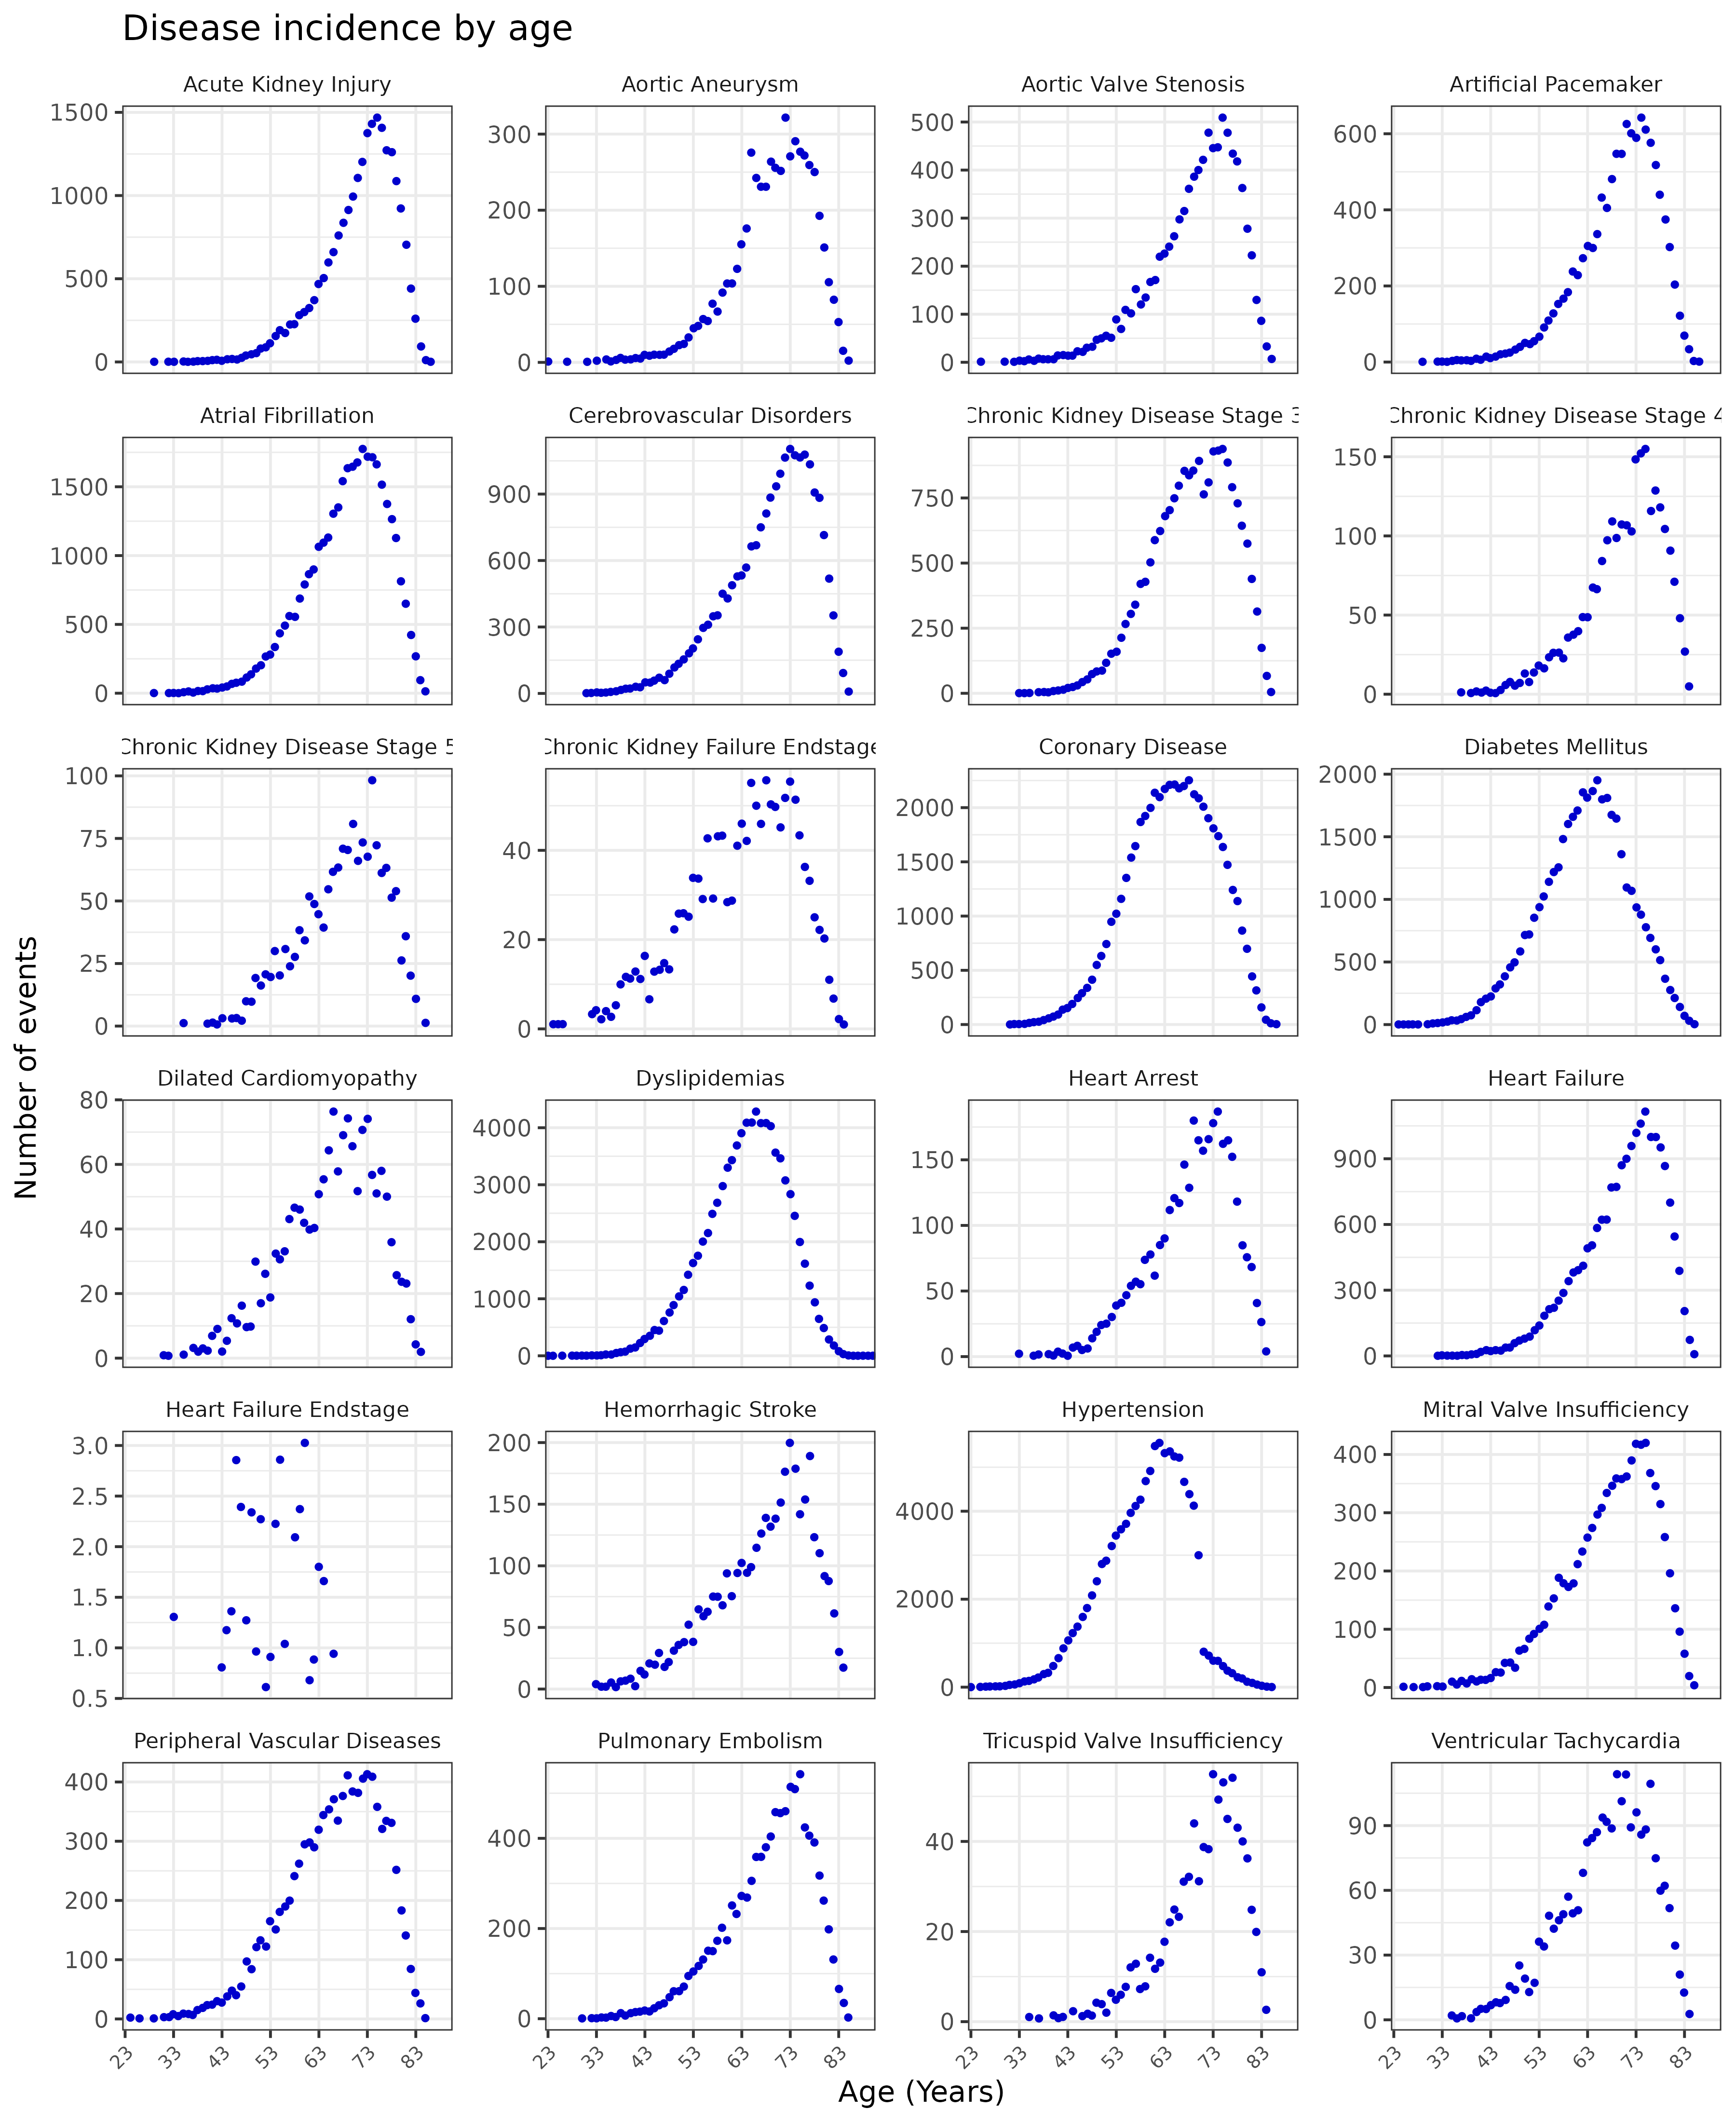
\includegraphics[width=0.8\textwidth]{Figures/disease_incidence_by_age.png}
    \caption{Age distribution of disease incidence across 24 primary diseases. Each panel shows the number of incident cases by age (in years) for a specific disease. The y-axis scale varies across panels to accommodate different incidence rates.}
    \label{supp_mat:SF0}
\end{figure}

\newpage

\begin{figure}[H]
    \centering
    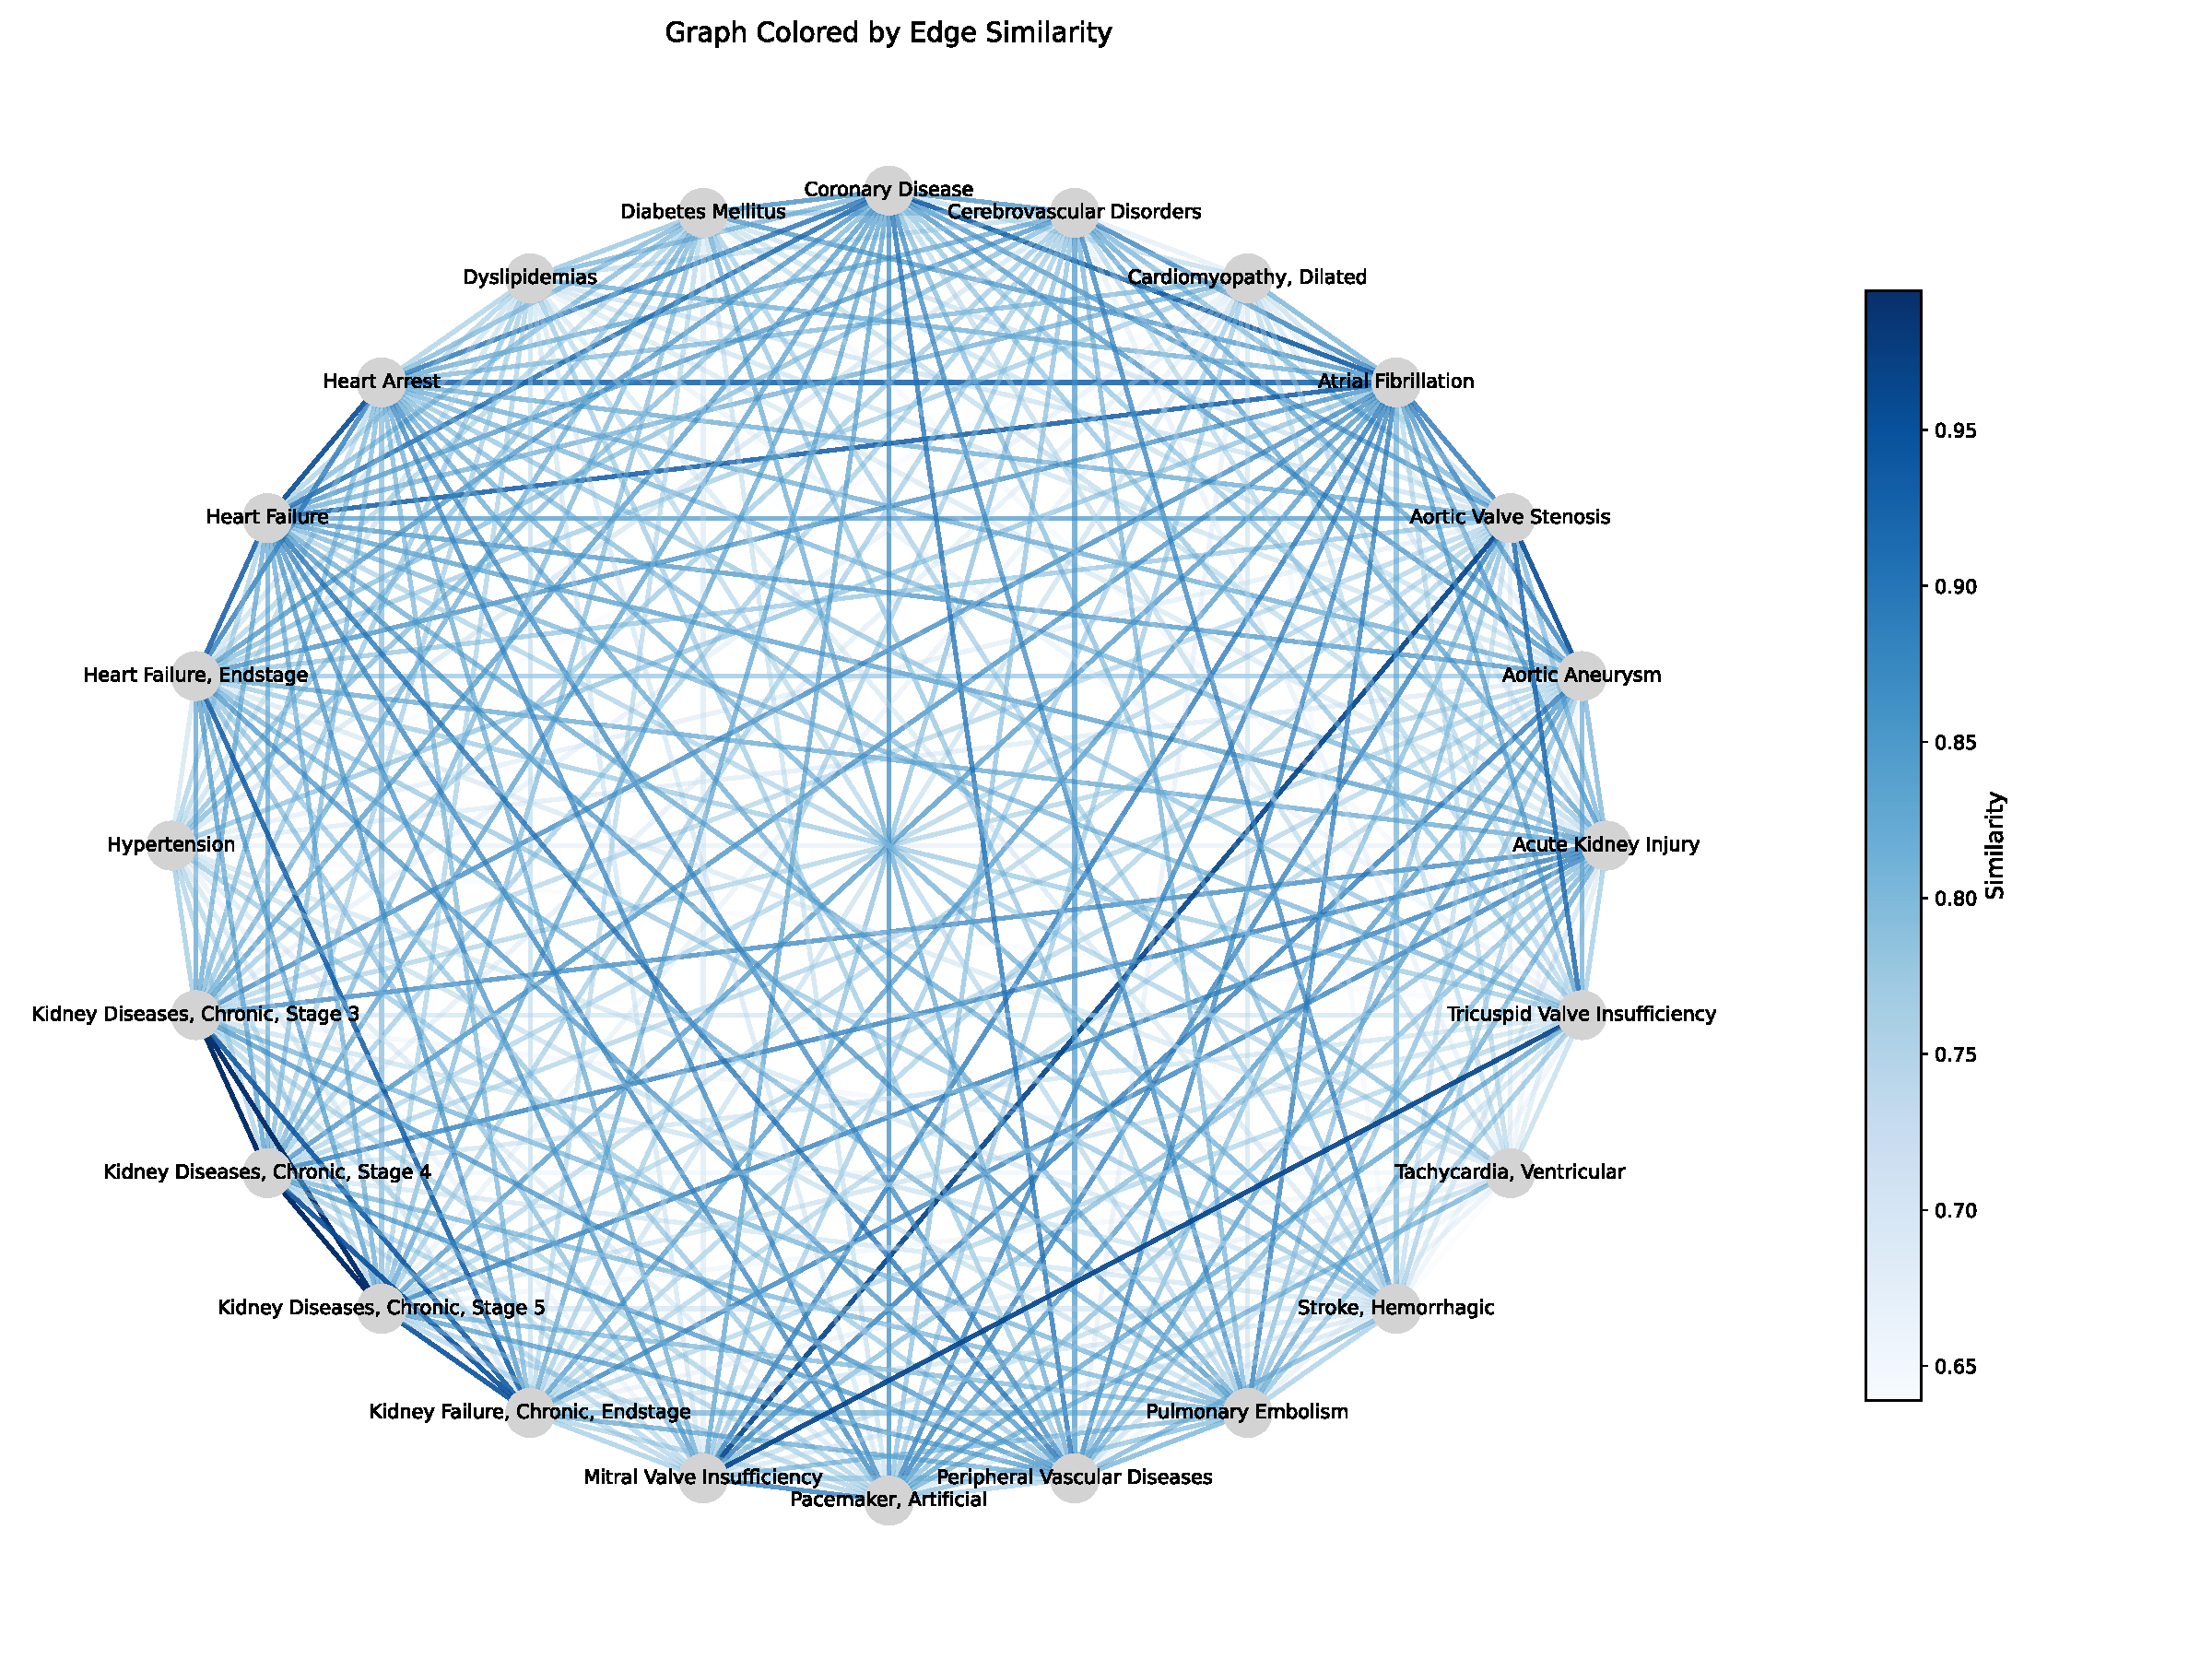
\includegraphics[width=1\textwidth]{Figures/graph_similarity_plot_main_par.pdf}
    \caption{Cosine similarity network for 24 cardiometabolic diseases computed from embeddings including both cardiometabolic diseases and risk factors. Darker colors indicate stronger similarities.}
    \label{supp_mat:SF2}
\end{figure}


\begin{figure}[H]
    \centering
    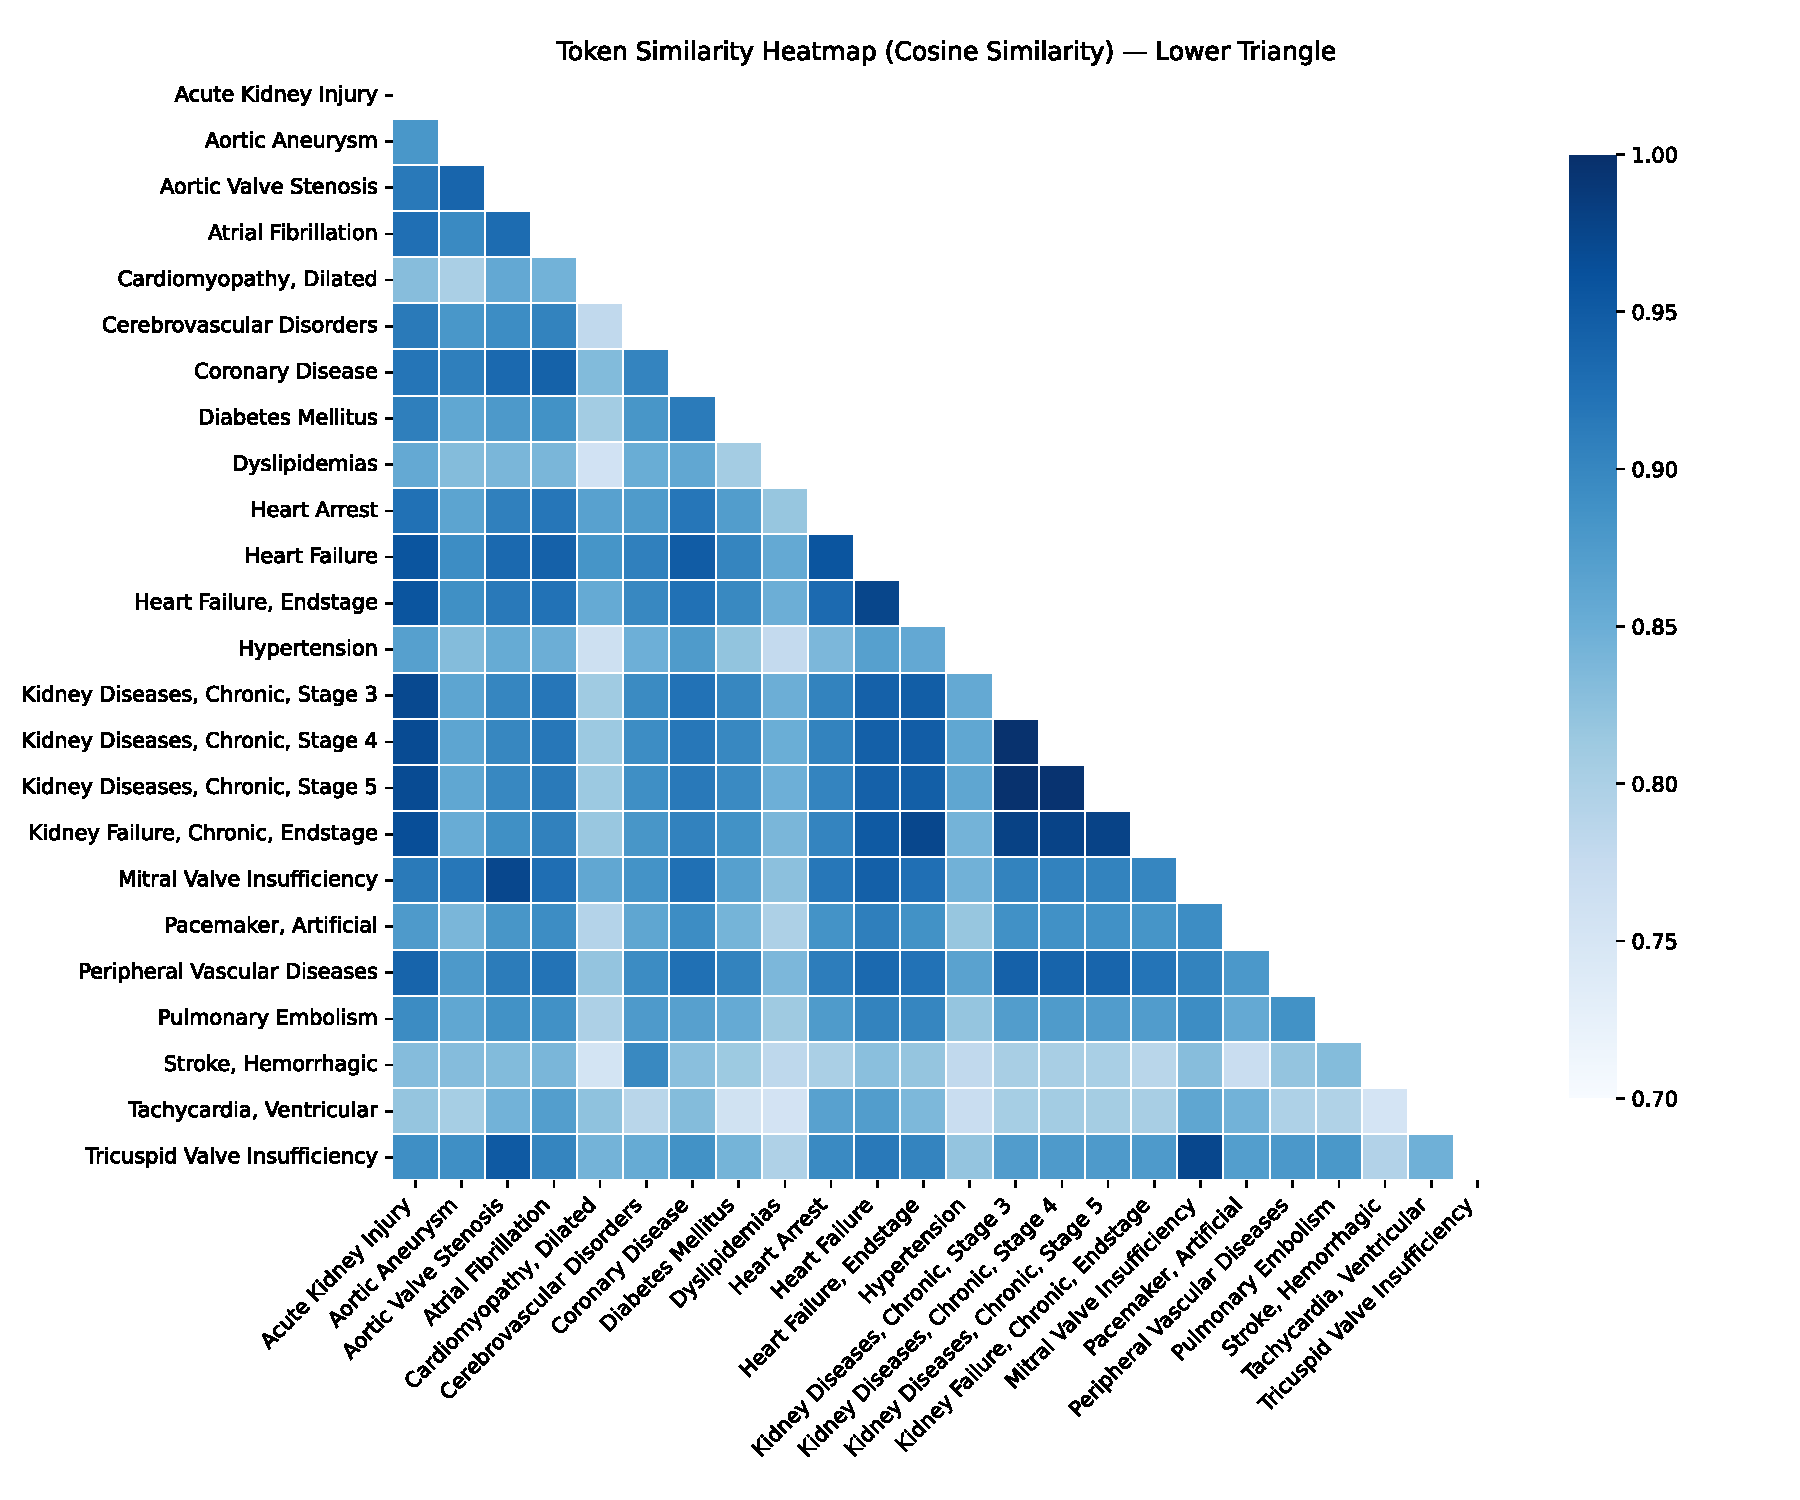
\includegraphics[width=1\textwidth]{Figures/disease_similarity_heatmap_main.pdf}
    \caption{Cosine similarity matrix for 24 cardiometabolic diseases computed from embeddings including only cardiometabolic diseases. Darker colors indicate stronger similarities.}
    \label{supp_mat:SF1}
\end{figure}



\newpage

\begin{figure}[H]
    \centering
    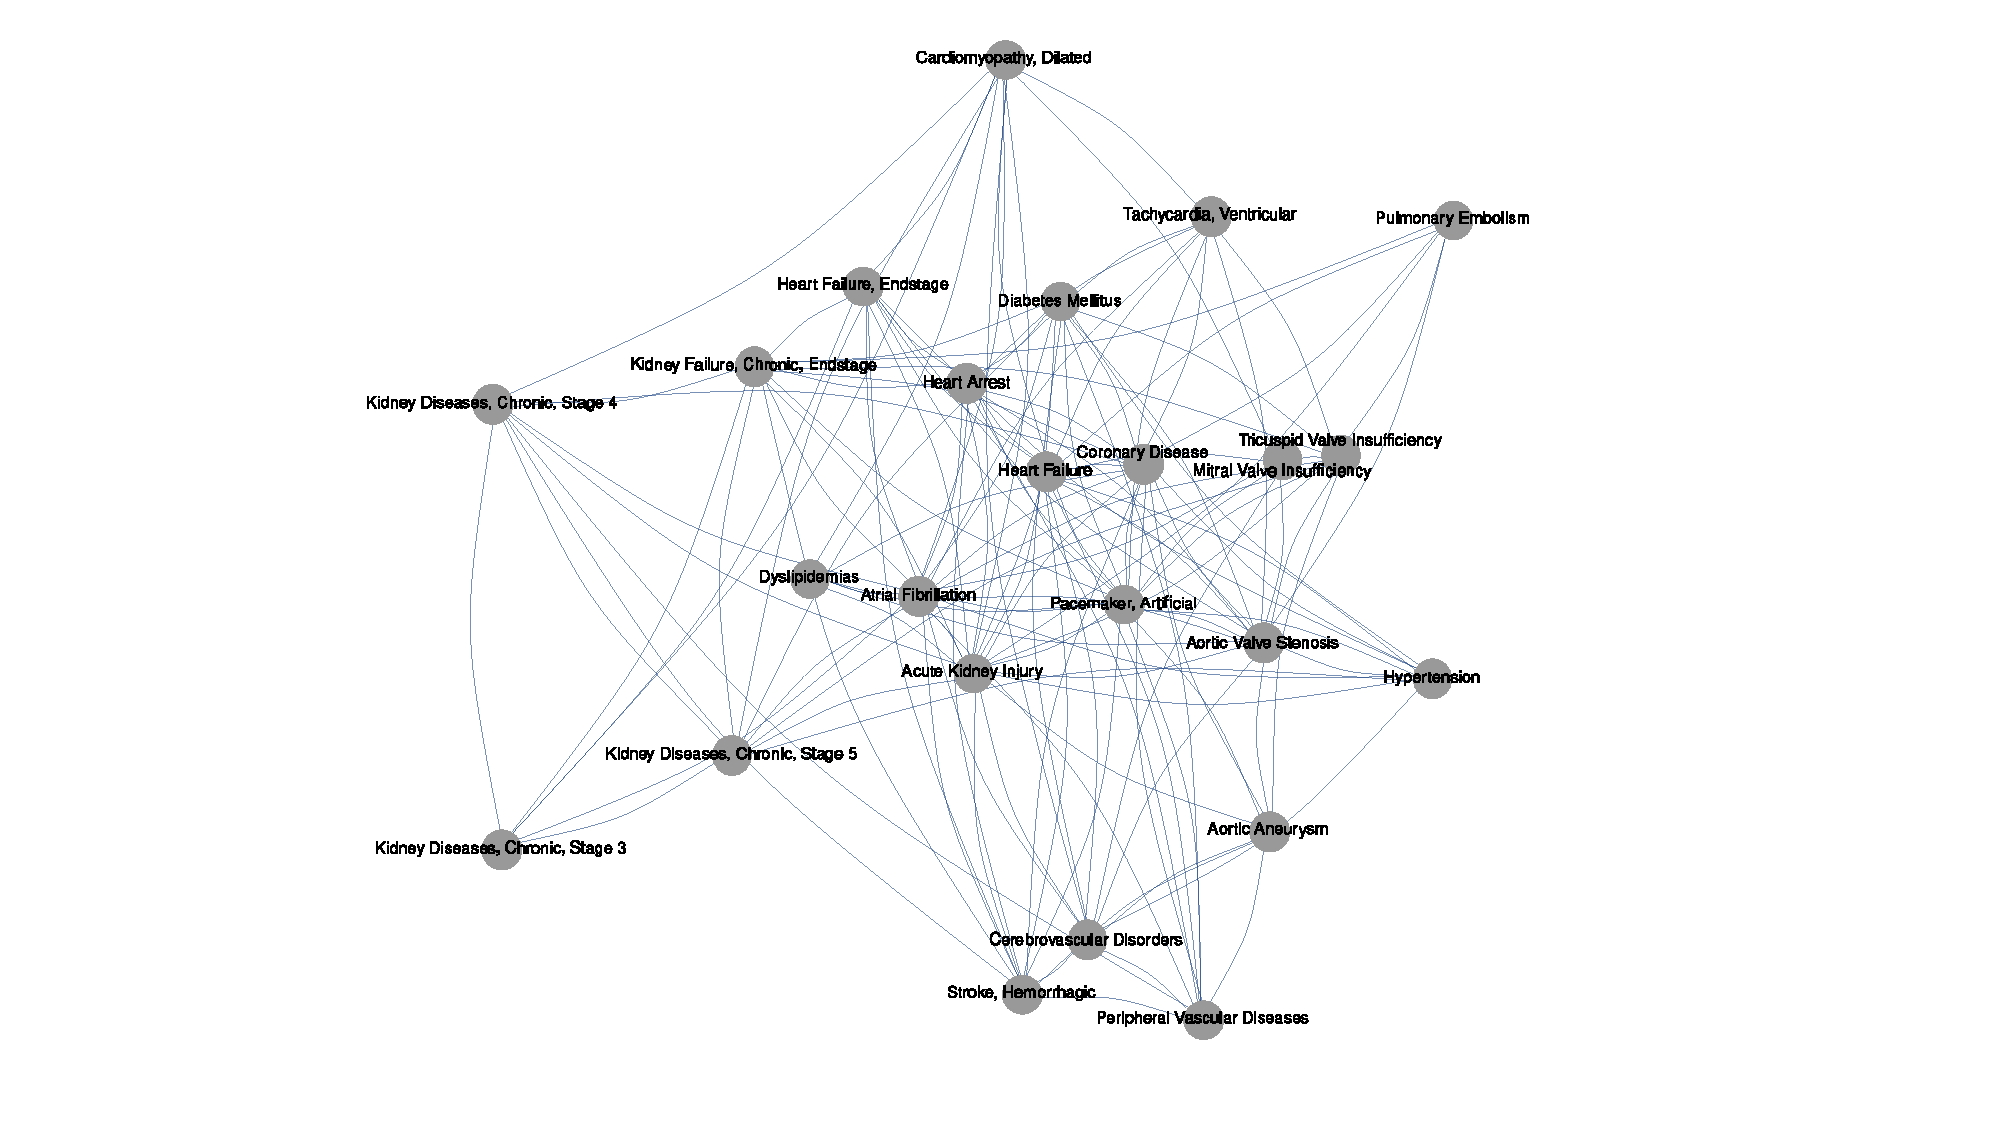
\includegraphics[width=1\textwidth]{Figures/Plots_graph_Baseline_HR.pdf}
    \caption{Cardiometabolic disease network estimated via Gaussian Graphical Lasso Regression computed from embeddings including both cardiometabolic diseases and risk factors.}
    \label{supp_mat:SF3}
\end{figure}

\clearpage

\bibliographystyle{biorefs}
\bibliography{bibliography}


\end{document}